\appendix
% Special numbering for appendix (Use "S" instead of "A" in Supplement)
\renewcommand{\thesection}{A\arabic{section}}
\renewcommand{\theequation}{A\arabic{equation}}
\renewcommand{\thetheorem}{A\arabic{theorem}}
\renewcommand{\thecorollary}{A\arabic{corollary}}
\renewcommand{\theproposition}{A\arabic{proposition}}
\renewcommand{\thelemma}{A\arabic{lemma}}
\renewcommand{\thetable}{A\arabic{table}}
\renewcommand{\thefigure}{A\arabic{figure}}
\renewcommand{\thealgorithm}{A\arabic{algorithm}}


% \setcounter{figure}{0}
% \setcounter{table}{0}
% \setcounter{proposition}{0}
% \setcounter{corollary}{0}
% \setcounter{theorem}{0}
% \setcounter{lemma}{0}
% \setcounter{algorithm}{0}



\section{Naive early stopping benchmarks} \label{app:naive-benchmarks}

\subsection{Detailed implementation of the naive benchmarks}  \label{app:naive-benchmarks-details}

We detail here the implementation of the naive benchmark considered in this paper, which consist of performing standard conformal calibration using the same hold-out samples utilized by standard early stopping techniques.
This does not yield theoretically valid conformal inferences in finite samples because greedily utilizing the same hold-out data set twice, both to evaluate the early stopping criterion and to perform conformal calibration, will break the necessary exchangeability with the test point. Nonetheless, this approach can serve as an informative benchmark and it becomes useful in Appendix~\ref{app:reg-noempty} to extend our rigorous conformalized early stopping method for regression problems in such as way as to explicitly avoid returning empty prediction intervals.
For completeness, we present the implementation of the naive benchmark separately for outlier detection, multi-class classification, and regression, respectively in Algorithms~\ref{alg:naive-one}, \ref{alg:naive-multi} and~\ref{alg:naive-reg}.
Note that Algorithm~\ref{alg:naive-multi} also allows for the possibility of computing prediction sets seeking (approximate) marginal coverage instead of (approximate) label-conditional coverage for multi-class classification problems; see Appendix~\ref{app:class-marg} for further details on multi-class classification with marginal coverage.

\begin{algorithm}[H]
    \caption{Naive conformal outlier detection benchmark with greedy early stopping}
    \label{alg:naive-one}
    \begin{algorithmic}[1]
        \STATE \textbf{Input}: Exchangeable data points $Z_1, \ldots, Z_n$; test point $Z_{n+1}$.
        \STATE \textcolor{white}{\textbf{Input}:} Maximum number of training epochs $t^{\max}$; storage period hyper-parameter $\tau$.
        \STATE \textcolor{white}{\textbf{Input}:} One-class classifier trainable via (stochastic) gradient descent.
        \STATE Randomly split the exchangeable data points into $\mathcal{D}_{\text{train}}$ and $\mathcal{D}_{\text{es-cal}}$.
        \STATE Train the one-class classifier for $t^{\text{max}}$ epochs and save the intermediate models $M_{t_1} , \dots, M_{t_T}$.
        \STATE Pick the most promising model $t^* \in [T]$ minimizing $\mathcal{L}_{\text{es-cal}}(M_t)$ in \eqref{eq:loss-ces}, using the data in $\mathcal{D}_{\text{es-cal}}$.
        \STATE Compute nonconformity scores $\hat{S}_i(Z_{n+1})$ for all $i \in \mathcal{D}_{\text{es-cal}} \cup \{n+1\}$ using model $t^*$.
        \STATE \textbf{Output}: Naive conformal p-value $\hat{u}_0^{\textup{naive}}(Z_{n+1})$ given by \eqref{eq:conformal_pval}.
    \end{algorithmic}
\end{algorithm}

\begin{algorithm}[H]
    \caption{Naive conformal multi-class classification benchmark with greedy early stopping}
    \label{alg:naive-multi}
    \begin{algorithmic}[1]
        \STATE \textbf{Input}: Exchangeable data points $(X_{1},Y_{1}), \ldots, (X_{n},Y_{n}), (X_{n+1},Y_{n+1})$ with labels $Y_i \in [K]$.
        \STATE \textcolor{white}{\textbf{Input}:} Test point with features $X_{n+1}$. Desired coverage level $1-\alpha$.
        \STATE \textcolor{white}{\textbf{Input}:} Maximum number of training epochs $t^{\max}$; storage period hyper-parameter $\tau$.
        \STATE \textcolor{white}{\textbf{Input}:} $K$-class classifier trainable via (stochastic) gradient descent.
        \STATE Randomly split the exchangeable data points into $\mathcal{D}_{\text{train}}$ and $\mathcal{D}_{\text{es-cal}}$.
        \STATE Train the $K$-class classifier for $t^{\text{max}}$ epochs and save the intermediate models $M_{t_1} , \dots, M_{t_T}$.
        \STATE Pick the most promising model $t^* \in [T]$ minimizing $\mathcal{L}_{\text{es-cal}}(M_t)$ in \eqref{eq:loss-ces-class}, using the data in $\mathcal{D}_{\text{es-cal}}$.
        \FOR{$ y \in [K]$}
        \IF{Label-conditional coverage is desired}
        \STATE Define $\mathcal{D}^y_{\text{es-cal}} = \{i \in \mathcal{D}_{\text{es-cal}} : Y_i = y \}$.
        \STATE Compute scores $\hat{S}_i^y(X_{n+1})$ for all $i \in \mathcal{D}^y_{\text{es-cal}} \cup \{n+1\}$ using model $t^*$; see Appendix~\ref{app:class-scores}.
        \STATE Compute the naive conformal p-value $\hat{u}^{\textup{naive}}_y(X_{n+1})$ according to \eqref{eq:conformal_pval-class}.
        \ELSE
        \STATE Compute scores $\hat{S}_i^y(X_{n+1})$ for all $i \in \mathcal{D}_{\text{es-cal}} \cup \{n+1\}$ using model $t^*$; see Appendix~\ref{app:class-scores}.
        \STATE Compute the naive conformal p-value $\hat{u}^{\textup{naive}}_y(X_{n+1})$ according to
        \begin{align*}
          \hat{u}^{\textup{naive}}_y(X_{n+1}) = \frac{1 + |i \in \mathcal{D}_{\text{es-cal}}: \hat{S}_{i}^y(X_{n+1}) \leq \hat{S}_{n+1}^y(X_{n+1})|}{1+|\mathcal{D}_{\text{es-cal}}|}.
        \end{align*}
        \ENDIF
        \ENDFOR

        \STATE \textbf{Output}: Naive prediction set $\hat{C}^{\textup{naive}}_{\alpha}(X_{n+1})$ given by \eqref{eq:pred-set-class}.
    \end{algorithmic}
\end{algorithm}


\begin{algorithm}[H]
    \caption{Naive conformal regression benchmark with greedy early stopping}
    \label{alg:naive-reg}
    \begin{algorithmic}[1]
        \STATE \textbf{Input}: Exchangeable data points $(X_{1},Y_{1}), \ldots, (X_{n},Y_{n}), (X_{n+1},Y_{n+1})$ with outcomes $Y_i \in \mathbb{R}$.
        \STATE \textcolor{white}{\textbf{Input}:} Test point with features $X_{n+1}$. Desired coverage level $1-\alpha$.
        \STATE \textcolor{white}{\textbf{Input}:} Maximum number of training epochs $t^{\max}$; storage period hyper-parameter $\tau$.
        \STATE \textcolor{white}{\textbf{Input}:} Regression model trainable via (stochastic) gradient descent.
        \STATE Randomly split the exchangeable data points into $\mathcal{D}_{\text{train}}$ and $\mathcal{D}_{\text{es-cal}}$.
        \STATE Train the regression model for $t^{\text{max}}$ epochs and save the intermediate models $M_{t_1} , \dots, M_{t_T}$.
        \STATE Pick the most promising model $t^* \in [T]$ minimizing $\mathcal{L}_{\text{es-cal}}(M_t)$ in \eqref{eq:loss-ces-reg}.
        \STATE Evaluate nonconformity scores $\hat{S}_i(X_{n+1}) = | Y_i - \hat{\mu}_{t^*}(X_{i})|$ for all $i \in \mathcal{D}_{\text{es-cal}}$.
        \STATE Compute $\hat{Q}_{1-\alpha}(X_{n+1}) = \lceil (1-\alpha)(1+|\mathcal{D}_{\text{es-cal}}|) \rceil\text{-th largest value in }
        \hat{S}_i(X_{n+1})$ for $i \in \mathcal{D}_{\text{es-cal}}$.
        \STATE \textbf{Output}: Naive prediction interval $\hat{C}^{\text{naive}}_{\alpha}(X_{n+1}) = \hat{\mu}_{t^*}(X_{n+1}) \pm \hat{Q}_{1-\alpha}(X_{n+1})$.
    \end{algorithmic}
\end{algorithm}


\begin{algorithm}[H]
    \color{blue}
    \caption{Naive conformal quantile regression benchmark with greedy early stopping}
    \label{alg:naive-reg-cqr}
    \begin{algorithmic}[1]
        \STATE \textbf{Input}: Quantiles = [$\beta_{\text{low}}, \beta_{\text{high}}$]. Exchangeable data points $(X_{1},Y_{1}), \ldots, (X_{n},Y_{n}), (X_{n+1},Y_{n+1})$ with outcomes $Y_i \in \mathbb{R}$.
        \STATE \textcolor{white}{\textbf{Input}:} Test point with features $X_{n+1}$. Desired coverage level $1-\alpha$.
        \STATE \textcolor{white}{\textbf{Input}:} Maximum number of training epochs $t^{\max}$; storage period hyper-parameter $\tau$.
        \STATE \textcolor{white}{\textbf{Input}:} Quantile egression model trainable via (stochastic) gradient descent minimizing the pinball loss.
        \STATE Randomly split the exchangeable data points into $\mathcal{D}_{\text{train}}$ and $\mathcal{D}_{\text{es-cal}}$.
        \STATE Train the quantile regression models for $t^{\text{max}}$ epochs and save the intermediate models $M_{\beta_{\text{low}},t_1} , \dots, M_{\beta_{\text{low}}t_T}$,  $M_{\beta_{\text{high}},t_1} , \dots, M_{\beta_{\text{high}}t_T}$.
        \STATE Pick the most promising models $t^*_{\text{low}}, t^*_{\text{high}}\in [T]$ minimizing $\mathcal{L}_{\text{es-cal}}(M_t)$ in \eqref{eq:loss-ces-reg-cqr}.
        \STATE Evaluate nonconformity scores $\hat{E}_i(X_{n+1}) = \max\{\hat{q}_{t^*_{\text{low}}}(X_i) - Y_i, Y_i -\hat{q}_{t^*_{\text{high}}}(X_i)\}$ for all $i \in \mathcal{D}_{\text{es-cal}}$.
        \STATE Compute $\hat{Q}_{1-\alpha}(X_{n+1}) = \lceil (1-\alpha)(1+|\mathcal{D}_{\text{es-cal}}|) \rceil\text{-th largest value in }
        \hat{E}_i(X_{n+1})$ for $i \in \mathcal{D}_{\text{es-cal}}$.
        \STATE \textbf{Output}: Naive prediction interval $\hat{C}^{\text{naive}}_{\alpha}(X_{n+1}) = [\hat{q}_{t^*_{\text{low}}}(X_{n+1}) - \hat{Q}_{1-\alpha}(X_{n+1}), \hat{q}_{t^*_{\text{high}}}(X_{n+1}) + \hat{Q}_{1-\alpha}(X_{n+1})]$.
    \end{algorithmic}
\end{algorithm}


\subsection{Theoretical analysis of the naive benchmark} \label{app:naive-analysis}

Although the naive benchmarks described above often perform similarly to CES in practice, they do not enjoy the same desirable theoretical guarantees.
Nonetheless, we can study their behaviour in sufficient detail as to prove that their inferences are too far from being valid.
Unfortunately, as demonstrated in Section~\ref{sec:numerical_results}, these theoretical results are still not tight enough to be very useful in practice.
For simplicity, we will begin by focusing on outlier detection.


\noindent \textbf{Review of existing results based on the DKW inequality.}
\citet{efficiency_first_cp} have recently studied the finite-sample coverage rate of a conformal prediction interval formed by naively calibrating a model selected among $T$ possible candidates based on its performance on the calibration data set itself, which we denote by $\mathcal{D}_{\text{es-cal}}$.
Although \citet{efficiency_first_cp} focus on conformal prediction intervals, here we find it easier to explain their ideas in the context of conformal p-values for outlier detection.

Let $\hat{S}_i(Z_{n+1};t)$, for all $i \in \mathcal{D}_{\text{es-cal}}$ and $t \in [T]$, denote the nonconformity scores corresponding to model $t$, and denote the  $\lfloor \alpha(1+|\mathcal{D}_{\text{es-cal}}|) \rfloor\text{-th largest value in }\hat{S}_i(X_{n+1};t)$ as $\hat{Q}_{\alpha}(Z_{n+1};t)$.
Let $t^*$  indicate the selected model.
As we are interested in constructing a conformal p-value $\hat{u}_0^{\textup{naive}}(Z_{n+1})$, the goal is to bound from above the tail probability
\begin{align}
    \mathbb{P}\left( \hat{u}_0^{\textup{naive}}(Z_{n+1}) > \alpha \right) = \mathbb{E} \left[  \mathbb{P} \left( \hat{S}_i(X_{n+1};t^*)> \hat{Q}_{\alpha}(Z_{n+1};t^*) \mid \mathcal{D}_{\text{es-cal}}\right) \right].
\end{align}
Intuitively, if $n_{\text{es-cal}} = |\mathcal{D}_{\text{es-cal}}|$ is sufficiently large, the conditional probability inside the expected value on the right-hand-side above can be well-approximated by the following empirical quantity:
\begin{align*}
    \frac{1}{n}\sum_{i \in \mathcal{D}_{\text{es-cal}}} \mathbbm{1} \left\{ \hat{S}_i(X_{n+1};t^*) > \hat{Q}_{\alpha}(Z_{n+1};t^*) \right \} = \frac{\lceil (1+n_{\text{es-cal}})(1-\alpha) \rceil}{n_{\text{es-cal}}} \geq \left( 1+\frac{1}{n_{\text{es-cal}}}\right)(1-\alpha).
\end{align*}
The quality of this approximation in finite samples can be bound by the DKW inequality, which holds for any $\varepsilon \geq 0$:
\begin{align}
    \mathbb{P}\left( \sup_{s \in \mathbb{R}} \left| \frac{1}{n_{\text{es-cal}}}\sum_{i \in \mathcal{D}_{\text{es-cal}}} \mathbbm{1} \left\{\hat{S}_i(X_{n+1};t^*) > s \right \} -  \mathbb{P} \left( \hat{S}_i(X_{n+1};t^*)> s \mid \mathcal{D}_{\text{es-cal}}\right)\right| > \varepsilon \right) \leq 2 e^{-2 n_{\text{es-cal}} \varepsilon^2}.
\end{align}
Starting from this, Theorem 1 in \citet{efficiency_first_cp} shows that
\begin{align}
     \mathbb{P}(\hat{u}_0^{\textup{naive}}(Z_{n+1}) > \alpha) \geq \left(1+\frac{1}{n_{\text{es-cal}}} \right)(1-\alpha)-\frac{\sqrt{\log(2T)/2}+c(T)}{\sqrt{n_{\text{es-cal}}}},
\end{align}
where $c(T)$ is a constant that can be computed explicitly and is generally smaller than $1/3$.
Intuitively, the $[\sqrt{\log(2T)/2}+c(T)]/ \sqrt{n_{\text{es-cal}}}$ term above can be interpreted as the worst-case approximation error among all possible models $t \in [T]$.

One limitation with this result is that is gives a worst-case correction that does not depend on the chosen level $\alpha$, and one would intuitively expect this bound to be tighter for $\alpha = 1/2$ and overly conservative for the small $\alpha$ values (e.g., $\alpha = 0.1$) that are typically interesting in practice. (This intuition will be confirmed empirically in Figure~\ref{fig:bound_alpha}.)
This observation motivates the following alternative analysis, which can often give tighter results.


\noindent \textbf{Alternative probabilistic bound based on Markov's inequality.}
Define $W_t=\P{\hat{u}_0^{\textup{naive}}(Z_{n+1};t) > \alpha \mid \mathcal{D}_{\text{es-cal}}}$. Lemma~3 in \citet{vovk2012conditional} tells us that $W_t$ follows a Beta distribution, assuming exchangeability among $\mathcal{D}_{\text{es-cal}}$ and the test point. That is,
\begin{align*}
    W_t \sim \text{Beta}(n_{\text{es-cal}}+1-l, l), \hspace{10pt} l=\lfloor \alpha(n_{\text{es-cal}}+1) \rfloor.
\end{align*}
In the following, we will denote the corresponding inverse Beta cumulative distribution function as $I^{-1}(x;n_{\text{es-cal}}+1-l,l)$.
This result can be used to derive an alternative upper bound for $\mathbb{P}(\hat{u}_0^{\textup{naive}}(Z_{n+1}) > \alpha)$ using the Markov's inequality.

\begin{proposition}\label{prop:naive-od}
    Assume $Z_{1}, \ldots, Z_{n}, Z_{n+1}$ are exchangeable random samples, and let $\hat{u}^{\textup{naive}}_0(Z_{n+1})$ be the output of Algorithm~\ref{alg:naive-one}, for any given $\alpha \in (0,1)$. Suppose Algorithm~\ref{alg:naive-one} is based on a learning algorithm that is invariant to permutations of the training data.
Then, for any fixed $\alpha \in (0,1)$ and any $b>1$, letting $l=\lfloor \alpha(n_{\text{es-cal}}+1)  \rfloor$,
$$\P{\hat{u}^{\textup{naive}}_0(Z_{n+1}) > \alpha} \geq I^{-1}\left( \frac{1}{bT};n_{\text{es-cal}}+1-l,l \right) \cdot (1-1/b).$$
\end{proposition}

Note that the bound given by Proposition~\ref{prop:naive-od} depends on $\alpha$ in a more complex way and does not have an explicit analytical form, unlike that of \citet{efficiency_first_cp}. However, this Markov bound is easy to compute numerically and often turns out to be tighter as long as $b$ is moderately large (e.g., $b=100$), as we shall see below.
Naturally, the same idea can also be applied to bound the coverage of naive conformal prediction sets or intervals output by Algorithm~\ref{alg:naive-multi} or Algorithm~\ref{alg:naive-reg}, respectively.


\begin{corollary} \label{prop:naive-class}
    Assume $(X_1,Y_1), \ldots, (X_n,Y_n), (X_{n+1},Y_{n+1})$ are exchangeable random sample, and let $\hat{C}_{\alpha}^{\textup{naive}}(X_{n+1})$ be the output of Algorithm~\ref{alg:naive-multi}, for any given $\alpha \in (0,1)$. Suppose Algorithm~\ref{alg:naive-multi} is based on a learning algorithm that is invariant to permutations of the training data. Then, for any $b > 1$, letting $l=\lfloor \alpha(n_{\text{es-cal}}+1) \rfloor$, $$\P{Y_{n+1} \in \hat{C}^{\textup{naive}}_{\alpha}(X_{n+1})} \geq I^{-1}\left(\frac{1}{bT}; n_{\text{es-cal}}+1-l,l\right) \cdot (1-1/b).$$
\end{corollary}


\begin{corollary}\label{prop:naive-reg}
Assume $(X_{1},Y_{1}), \ldots, (X_{n},Y_{n}), (X_{n+1},Y_{n+1})$ are exchangeable random samples, and let $\hat{C}^{\textup{naive}}_{\alpha}(X_{n+1})$ be the output of Algorithm~\ref{alg:naive-reg}, for any $\alpha \in (0,1)$. Suppose Algorithm~\ref{alg:naive-reg} is based on a learning algorithm that is invariant to permutations of the training data. Then, for any $b > 1$, letting $l=\lfloor \alpha(n_{\text{es-cal}}+1) \rfloor$,
$$\P{Y_{n+1} \in \hat{C}^{\textup{naive}}_{\alpha}(X_{n+1})} \geq I^{-1}\left(\frac{1}{bT}; n_{\text{es-cal}}+1-l,l\right) \cdot (1-1/b).$$
\end{corollary}


\noindent \textbf{Hybrid probabilistic bound.}
Since neither the DKW nor the Markov bound described above always dominate the other for all possible combinations of $T$, $n_{\text{es-cal}}$, and $\alpha$, it makes sense to combine them to obtain a uniformly tighter {\em hybrid} bound.
For any fixed $b>1$ and any $T$, $n_{\text{es-cal}}$, and $\alpha$, define $H(T,n_{\text{es-cal}},\alpha)$ as
%Now we compare the DKW bound and Markov bound from the numerical aspect. From Figure~\ref{fig:bound_tn}, we can see that the Markov bound decays slower when the model sizes grows, but the DKW bound performs better when the calibration size $n$ is big enough. This inspires us to combine the two bounds by taking the maximum, formally, we define the new hybrid bound by:
\begin{align*}
    H(T,n_{\text{es-cal}},\alpha)
  = \max\left\{ I^{-1} \left(\frac{1}{bT}; n_{\text{es-cal}}+1-l,l \right) \cdot (1-1/b), \left(1+\frac{1}{n_{\text{es-cal}}}\right)(1-\alpha)-\frac{\sqrt{\log(2T)/2}+c(T)}{\sqrt{n_{\text{es-cal}}}} \right\}.
\end{align*}
It then follows immediately from \citet{efficiency_first_cp} and Proposition~\ref{prop:naive-od} that, under the same conditions of Proposition~\ref{prop:naive-od}, for any  fixed $b>1$,
$$\P{\hat{u}^{\textup{naive}}_0(Z_{n+1}) > \alpha} \geq H(T,n_{\text{es-cal}},\alpha).$$
Of course, the same argument can also be utilized to tighten the results of Corollaries~\ref{prop:naive-class}--\ref{prop:naive-reg}.

\noindent \textbf{Numerical comparison of different probabilistic bounds.}
Figure~\ref{fig:bound_tn} compares the three probabilistic bounds described above ({\em DKW}, {\em Markov}, and {\em hybrid}) as a function of the number of candidate models $T$ and of the number of hold-out data points $n_{\text{es-cal}}$, in the case of $\alpha=0.1$. For simplicity, the Markov and hybrid bounds are evaluated by setting $b=100$, which may not be the optimal choice but appears to work reasonably well. These results show that Markov bound tends to be tighter than the DKW bound for large values of $T$ and for small values of $n_{\text{es-cal}}$, while the hybrid bound generally achieves the best of both worlds.
Lastly, Figure~\ref{fig:bound_alpha} demonstrates that the Markov bound tends to be tighter when $\alpha$ is small. The Markov and hybrid bounds here are also evaluated using $b=100$.

\begin{figure}
    \centering
    \includegraphics[scale=0.63]{diagrams/bound_comparison1.png}
    \caption{Numerical comparison of different theoretical lower bounds for the marginal coverage of conformal prediction sets computed with a naive early stopping benchmark (e.g., Algorithm~\ref{alg:naive-multi}). Left: lower bounds for the marginal coverage as a function of the number of candidate models $T$, when $\alpha=0.1$ and $n_{\text{es-cal}}=8000$.
Right: lower bounds for the marginal coverage as a function of the number of hold-out data points, $n_{\text{es-cal}}$, when $\alpha=0.1$ and $T=100$. Higher values correspond to tighter bounds.
}
    \label{fig:bound_tn}
\end{figure}


\begin{figure}
    \centering
    \includegraphics[scale=0.63]{diagrams/bound_comparison2.png}
    \caption{Numerical comparison of different theoretical lower bounds for the marginal coverage of conformal prediction sets computed with a naive early stopping benchmark (e.g., Algorithm~\ref{alg:naive-multi}), as a function of the nominal significance level $\alpha$. Left: lower bounds for the marginal coverage as a function of $\alpha$, when $T = 1000$ and $n_{\text{es-cal}}= 1000$.
Right: theoretically corrected significance level necessary needed to achieve the marginal coverage guarantees expected at the nominal $\alpha$ level, as a function of $\alpha$ when $T = 1000$ and $n_{\text{es-cal}}= 1000$. The dashed grey lines indicate the ideal values corresponding to standard conformal inferences based on calibration data that are independent of those used for early stopping. Higher values correspond to tighter bounds.
}
    \label{fig:bound_alpha}
\end{figure}


\section{Main algorithms} \label{app:algorithms}

\begin{algorithm}[H]
    \caption{Conformalized early stopping for outlier detection}
    \label{alg:od_full_seq}
    \begin{algorithmic}[1]
        \STATE \textbf{Input}: Exchangeable data points $Z_1, \ldots, Z_n$; test point $Z_{n+1}$.
        \STATE \textcolor{white}{\textbf{Input}:} Maximum number of training epochs $t^{\max}$; storage period hyper-parameter $\tau$.
        \STATE \textcolor{white}{\textbf{Input}:} One-class classifier trainable via (stochastic) gradient descent.
        \STATE Randomly split the exchangeable data points into $\mathcal{D}_{\text{train}}$ and $\mathcal{D}_{\text{es-cal}}$.
        \STATE Train the one-class classifier for $t^{\text{max}}$ epochs and save the intermediate models $M_{t_1} , \dots, M_{t_T}$.
        \STATE Pick the most promising model $\hat{M}_{\text{ces}}(Z_{n+1})$ according to~\eqref{eq:ces-model}, using the data in $\mathcal{D}_{\text{es-cal}} \cup \{n+1\}$.
        \STATE Compute nonconformity scores $\hat{S}_i(Z_{n+1})$ for all $i \in \mathcal{D}_{\text{es-cal}} \cup \{n+1\}$ using model $\hat{M}_{\text{ces}}(Z_{n+1})$.
        \STATE \textbf{Output}: Conformal p-value $\hat{u}_0(Z_{n+1})$ given by \eqref{eq:conformal_pval}.
    \end{algorithmic}
\end{algorithm}

\begin{algorithm}[H]
    \caption{Conformalized early stopping for multi-class classification}
    \label{alg:class_full_seq}
    \begin{algorithmic}[1]
        \STATE \textbf{Input}: Exchangeable data points $(X_{1},Y_{1}), \ldots, (X_{n},Y_{n}), (X_{n+1},Y_{n+1})$ with labels $Y_i \in [K]$.
        \STATE \textcolor{white}{\textbf{Input}:} Test point with features $X_{n+1}$. Desired coverage level $1-\alpha$.
        \STATE \textcolor{white}{\textbf{Input}:} Maximum number of training epochs $t^{\max}$; storage period hyper-parameter $\tau$.
        \STATE \textcolor{white}{\textbf{Input}:} $K$-class classifier trainable via (stochastic) gradient descent.
        \STATE Randomly split the exchangeable data points into $\mathcal{D}_{\text{train}}$ and $\mathcal{D}_{\text{es-cal}}$.
        \STATE Train the $K$-class classifier for $t^{\text{max}}$ epochs and save the intermediate models $M_{t_1} , \dots, M_{t_T}$.
        \FOR{$ y \in [K]$}
        \STATE Define $\mathcal{D}^y_{\text{es-cal}} = \{i \in \mathcal{D}_{\text{es-cal}} : Y_i = y \}$ and imagine $Y_{n+1}=y$.
        \STATE Pick the model $\hat{M}_{\text{ces}}(X_{n+1},y)$ according to~\eqref{eq:ces-model-class}, using the data in $\mathcal{D}_{\text{es-cal}} \cup \{n+1\}$.
        \STATE Compute scores $\hat{S}_i^y(X_{n+1})$ for all $i \in \mathcal{D}^y_{\text{es-cal}} \cup \{n+1\}$ using $\hat{M}_{\text{ces}}(X_{n+1},y)$; see Appendix~\ref{app:class-scores}.
        \STATE Compute the conformal p-value $\hat{u}_y(X_{n+1})$ according to \eqref{eq:conformal_pval-class}.
        \ENDFOR
        \STATE \textbf{Output}: Prediction set $\hat{C}_{\alpha}(X_{n+1})$ given by \eqref{eq:pred-set-class}.
    \end{algorithmic}
\end{algorithm}

\begin{algorithm}[H]
    \caption{Conformalized early stopping for regression}
    \label{alg:reg}
    \begin{algorithmic}[1]
        \STATE \textbf{Input}: Exchangeable data points $(X_{1},Y_{1}), \ldots, (X_{n},Y_{n}), (X_{n+1},Y_{n+1})$ with outcomes $Y_i \in \mathbb{R}$.
        \STATE \textcolor{white}{\textbf{Input}:} Test point with features $X_{n+1}$. Desired coverage level $1-\alpha$.
        \STATE \textcolor{white}{\textbf{Input}:} Maximum number of training epochs $t^{\max}$; storage period hyper-parameter $\tau$.
        \STATE \textcolor{white}{\textbf{Input}:} Regression model trainable via (stochastic) gradient descent.
        \STATE Randomly split the exchangeable data points into $\mathcal{D}_{\text{train}}$ and $\mathcal{D}_{\text{es-cal}}$.
        \STATE Train the regression model for $t^{\text{max}}$ epochs and save the intermediate models $M_{t_1} , \dots, M_{t_T}$.
        \STATE Evaluate $\hat{M}_{\text{ces}}(X_{n+1},y)$ as in \eqref{eq:reg-step-func}, using Algorithm~\ref{alg:envelope}.
        \STATE Partition the domain of $Y$ into $L$ intervals $\mathcal{B}_l$, for $l \in [L]$, based on the knots of $\hat{M}_{\text{ces}}(X_{n+1},y)$.
        \FOR{$ l \in [L]$}
        \STATE Evaluate nonconformity scores $\hat{S}_i(X_{n+1},\mathcal{B}_l)$ for all $i \in \mathcal{D}_{\text{es-cal}}$ as in \eqref{eq:scores-reg}.
        \STATE Compute $\hat{Q}_{1-\alpha}(X_{n+1},\mathcal{B}_l)$ as the $\lceil (1-\alpha)(1+|\mathcal{D}_{\text{es-cal}}|) \rceil$-th largest value among $\hat{S}_i(X_{n+1},\mathcal{B}_l)$.
 \STATE Construct the interval $\hat{C}_{\alpha}(X_{n+1}, \mathcal{B}_l)$ according to~\eqref{eq:reg-int-tmp}.
%        \STATE Define $\mathcal{D}^y_{\text{es-cal}} = \{i \in \mathcal{D}_{\text{es-cal}} : Y_i = y \}$ and imagine $Y_{n+1}=y$.
%        \STATE Pick the model $\hat{M}_{\text{ces}}(X_{n+1},y)$ according to~\eqref{eq:ces-model-class}, using the data in $\mathcal{D}_{\text{es-cal}} \cup \{n+1\}$.
%        \STATE Compute scores $\hat{S}_i(X_{n+1},y)$ for all $i \in \mathcal{D}_{\text{es-cal}} \cup \{n+1\}$ using $\hat{M}_{\text{ces}}(X_{n+1},y)$; see Appendix~\ref{app:class-scores}.
%        \STATE Compute the conformal p-value $\hat{u}_y(X_{n+1})$ according to \eqref{eq:conformal_pval-class}.
        \ENDFOR
        \STATE \textbf{Output}: Prediction interval $\hat{C}_{\alpha}(X_{n+1})$ given as a function of $\{\hat{C}_{\alpha}(X_{n+1}, \mathcal{B}_l)\}_{l=1}^{L}$ by \eqref{eq:reg-int}.
    \end{algorithmic}
\end{algorithm}




\begin{algorithm}[H]
    \color{blue}
    \caption{Conformalized early stopping for quantile regression}
    \label{alg:reg-cqr}
    \begin{algorithmic}[1]
        \STATE \textbf{Input}: Quantiles = [$\beta_{\text{low}}$, $\beta_{\text{high}}$], Exchangeable data points $(X_{1},Y_{1}), \ldots, (X_{n},Y_{n}), (X_{n+1},Y_{n+1})$ with outcomes $Y_i \in \mathbb{R}$.
        \STATE \textcolor{white}{\textbf{Input}:} Test point with features $X_{n+1}$. Desired coverage level $1-\alpha$.
        \STATE \textcolor{white}{\textbf{Input}:} Maximum number of training epochs $t^{\max}$; storage period hyper-parameter $\tau$.
        \STATE \textcolor{white}{\textbf{Input}:} Quantile regression model trainable via (stochastic) gradient descent.
        \STATE Randomly split the exchangeable data points into $\mathcal{D}_{\text{train}}$ and $\mathcal{D}_{\text{es-cal}}$.
        \STATE Train the quantile regression model fors $t^{\text{max}}$ epochs and save the intermediate models $M_{\beta_{\text{low}}, t_1} , \dots, M_{\beta_{\text{low}}, t_T}$, $M_{\beta_{\text{high}}, t_1} , \dots, M_{\beta_{\text{high}}, t_T}$.
        \STATE Evaluate $\hat{M}_{\beta_{\text{low}},\text{ces}}(X_{n+1},y)$ and $\hat{M}_{\beta_{\text{high}},\text{ces}}(X_{n+1},y)$ as in \eqref{eq:reg-step-func-cqr-lowhigh}, using Algorithm~\ref{alg:envelope-cqr}.
        \STATE Partition the domain of $Y$ into $L_1+L_2$ intervals $\mathcal{B}_l$, for $l \in [L_1+L_2]$, based on the knots of $\hat{M}_{\beta_{\text{low}},\text{ces}}(X_{n+1},y)$ and $\hat{M}_{\beta_{\text{high}},\text{ces}}(X_{n+1},y)$.
        \FOR{$ l \in [L_1+ L_2]$}
        \STATE Evaluate nonconformity scores $\hat{E}_i(X_{n+1},\mathcal{B}_l)$ for all $i \in \mathcal{D}_{\text{es-cal}}$ as in \eqref{eq:scores-reg-cqr}.
        \STATE Compute $\hat{Q}_{1-\alpha}(X_{n+1},\mathcal{B}_l)$ as the $\lceil (1-\alpha)(1+|\mathcal{D}_{\text{es-cal}}|) \rceil$-th largest value among $\hat{E}_i(X_{n+1},\mathcal{B}_l)$.
 \STATE Construct the interval $\hat{C}_{\alpha}(X_{n+1}, \mathcal{B}_l)$ according to~\eqref{eq:reg-int-tmp-cqr}.
%        \STATE Define $\mathcal{D}^y_{\text{es-cal}} = \{i \in \mathcal{D}_{\text{es-cal}} : Y_i = y \}$ and imagine $Y_{n+1}=y$.
%        \STATE Pick the model $\hat{M}_{\text{ces}}(X_{n+1},y)$ according to~\eqref{eq:ces-model-class}, using the data in $\mathcal{D}_{\text{es-cal}} \cup \{n+1\}$.
%        \STATE Compute scores $\hat{S}_i(X_{n+1},y)$ for all $i \in \mathcal{D}_{\text{es-cal}} \cup \{n+1\}$ using $\hat{M}_{\text{ces}}(X_{n+1},y)$; see Appendix~\ref{app:class-scores}.
%        \STATE Compute the conformal p-value $\hat{u}_y(X_{n+1})$ according to \eqref{eq:conformal_pval-class}.
        \ENDFOR
        \STATE \textbf{Output}: Prediction interval $\hat{C}_{\alpha}(X_{n+1})$ given as a function of $\{\hat{C}_{\alpha}(X_{n+1}, \mathcal{B}_l)\}_{l=1}^{L}$ by \eqref{eq:reg-int-cqr}.
    \end{algorithmic}
\end{algorithm}


\section{Classification with marginal coverage} \label{app:class-marg}

The conformalized early stopping method presented in Section~\ref{sec:classification} can be easily modified to produce prediction sets with marginal rather than label-conditional coverage, as outlined in Algorithm~\ref{alg:class_full_seq_marg}.
The difference between Algorithm~\ref{alg:class_full_seq}  and Algorithm~\ref{alg:class_full_seq_marg} is that the latter utilizes all calibration data in $\mathcal{D}_{\text{es-cal}}$ to compute each conformal p-value $\hat{u}_y(X_{n+1})$, not only the samples with true label $y$.
An advantage of this approach is that conformal p-values based on a larger calibration samples are less aleatoric~\cite{bates2021testing} and require less conservative finite-sample corrections (i.e., the ``+1'' term the numerator of the p-value formula becomes more negligible as the calibration set size increases).
In turn, this tends to lead to smaller prediction sets with potentially more stable coverage conditional on the calibration data~\cite{sesia2020comparison,bates2021testing}
Of course, the downside of these prediction sets is that they can only be guaranteed to provide marginal coverage, although they can sometimes also perform well empirically in terms of label-conditional coverage~\cite{romano2020classification}.
\begin{theorem}\label{thm:class_full_marg}
Assume $(X_{1},Y_{1}), \ldots, (X_{n},Y_{n}), (X_{n+1},Y_{n+1})$ are exchangeable random samples, and let $\hat{C}_{\alpha}(X_{n+1})$ be the output of Algorithm~\ref{alg:class_full_seq_marg}, for any $\alpha \in (0,1)$. Suppose Algorithm~\ref{alg:class_full_seq_marg} is based on a multi-class classifier that is invariant to permutations of the training data. Then, $\mathbb{P}[Y_{n+1} \in \hat{C}_{\alpha}(X_{n+1})] \geq 1-\alpha$.
\end{theorem}



\begin{algorithm}[H]
    \caption{Conformalized early stopping for multi-class classification with marginal coverage}
    \label{alg:class_full_seq_marg}
    \begin{algorithmic}[1]
        \STATE \textbf{Input}: Exchangeable data points $(X_{1},Y_{1}), \ldots, (X_{n},Y_{n}), (X_{n+1},Y_{n+1})$ with labels $Y_i \in [K]$.
        \STATE \textcolor{white}{\textbf{Input}:} Test point with features $X_{n+1}$. Desired coverage level $1-\alpha$.
        \STATE \textcolor{white}{\textbf{Input}:} Maximum number of training epochs $t^{\max}$; storage period hyper-parameter $\tau$.
        \STATE \textcolor{white}{\textbf{Input}:} $K$-class classifier trainable via (stochastic) gradient descent.
        \STATE Randomly split the exchangeable data points into $\mathcal{D}_{\text{train}}$ and $\mathcal{D}_{\text{es-cal}}$.
        \STATE Train the $K$-class classifier for $t^{\text{max}}$ epochs and save the intermediate models $M_{t_1} , \dots, M_{t_T}$.
        \FOR{$ y \in [K]$}
        \STATE Imagine $Y_{n+1}=y$.
        \STATE Pick the model $\hat{M}_{\text{ces}}(X_{n+1},y)$ according to~\eqref{eq:ces-model-class}, using the data in $\mathcal{D}_{\text{es-cal}} \cup \{n+1\}$.
        \STATE Compute scores $\hat{S}_i(X_{n+1},y)$ for all $i \in \mathcal{D}_{\text{es-cal}} \cup \{n+1\}$ using $\hat{M}_{\text{ces}}(X_{n+1},y)$; see Appendix~\ref{app:class-scores}.
        \STATE Compute the conformal p-value $\hat{u}^{\text{marg}}_y(X_{n+1})$ according to
        \begin{align}\label{eq:conformal_pval-class_marg}
          \hat{u}^{\text{marg}}_y(X_{n+1}) = \frac{1 + |i \in \mathcal{D}_{\text{es-cal}}: \hat{S}_{i}^y(X_{n+1}) \leq \hat{S}_{n+1}^y(X_{n+1})|}{1+|\mathcal{D}_{\text{es-cal}}|}.
        \end{align}
        \ENDFOR
        \STATE \textbf{Output}: Prediction set $\hat{C}_{\alpha}(X_{n+1})$ given by \eqref{eq:pred-set-class}, with $\hat{u}^{\text{marg}}_y(X_{n+1})$ instead of $\hat{u}_y(X_{n+1})$.
    \end{algorithmic}
\end{algorithm}


\section{Review of nonconformity scores for classification} \label{app:class-scores}

This section reviews the relevant background on the adaptive nonconformity scores for classification developed by \citet{romano2020classification}.
For any $x \in \mathcal{X}$ and $y \in [K]$, let $\hat{\pi}_{y}(x)$ denote any (possibly very inaccurate) estimate of the true $\mathbb{P}[ Y = y \mid X =x]$ corresponding to the unknown data-generating distribution. Concretely, a typical choice of $\hat{\pi}$ may be given by the output of the final softmax layer of a neural network classifier, for example.
 For any $x \in \mathcal{X}$ and $\tau \in [0,1]$, define the \emph{generalized conditional quantile} function $L$, with input $x, \hat{\pi}, \tau$, as:
\begin{align} \label{eq:oracle-threshold}
  L(x; \hat{\pi}, \tau) & = \min \{ k \in [K] \ : \ \hat{\pi}_{(1)}(x) + \hat{\pi}_{(2)}(x) + \ldots + \hat{\pi}_{(k)}(x) \geq \tau \},
  \end{align}
where $\hat{\pi}_{(1)}(x) \leq \hat{\pi}_{(2)}(x) \leq \ldots \hat{\pi}_{(K)}(x)$ are the order statistics of $\hat{\pi}_{1}(x) \leq \hat{\pi}_{2}(x) \leq \ldots \hat{\pi}_{K}(x)$.
Intuitively, $L(x; \hat{\pi}, \tau)$ gives the size of the smallest possible subset of labels whose cumulative probability mass according to $\hat{\pi}$ is at least $\tau$.
Define also a function $\mathcal{S}$ with input $x$, $u \in (0,1)$, $\hat{\pi}$, and $\tau$ that computes the set of most likely labels up to (but possibly excluding) the one identified by $L(x; \hat{\pi}, \tau)$:
\begin{align} \label{eq:define-S}
    \mathcal{S}(x, u ; \hat{\pi}, \tau) & =
    \begin{cases}
    \text{ `$y$' indices of the $L(x ; \hat{\pi},\tau)-1$ largest $\hat{\pi}_{y}(x)$},
    & \text{ if } u \leq V(x ; \hat{\pi},\tau) , \\
    \text{ `$y$' indices of the $L(x ; \hat{\pi},\tau)$ largest $\hat{\pi}_{y}(x)$},
    & \text{ otherwise},
    \end{cases}
\end{align}
where
\begin{align*}
    V(x; \hat{\pi}, \tau) & =  \frac{1}{\hat{\pi}_{(L(x ; \hat{\pi}, \tau))}(x)} \left[\sum_{k=1}^{L(x ; \hat{\pi}, \tau)} \hat{\pi}_{(k)}(x) - \tau \right].
\end{align*}
Then, define the \textit{generalized inverse quantile} nonconformity score function $s$, with input $x,y,u;\hat{\pi}$, as:
\begin{align} \label{eq:define-scores}
    s(x,y,u;\hat{\pi}) & = \min \left\{ \tau \in [0,1] : y \in \mathcal{S}(x, u ; \hat{\pi}, \tau) \right\}.
\end{align}
Intuitively, $s(x,y,u;\hat{\pi})$ is the smallest value of $\tau$ for which the set $\mathcal{S}(x, u ; \hat{\pi}, \tau)$ contains the label $y$.
Finally, the nonconformity score for a data point $(X_i,Y_i)$ is given by:
\begin{align}
  \hat{S}_i
  & = s(X_i,Y_i,U_i;\hat{\pi}),
\end{align}
where $U_i$ is a uniform random variable independent of anything else. Note that this can also be equivalently written more explicitly as:
\begin{align}
  \hat{S}_i
  & = \hat{\pi}_{(1)}(X_i) + \hat{\pi}_{(2)}(X_i) + \ldots + \hat{\pi}_{(r(Y_i,\hat{\pi}(X_i)))}(X_i) - U_i\cdot \hat{\pi}_{(r(Y_i,\hat{\pi}(X_i)))}(X_i),
\end{align}
where $r(Y_i,\hat{\pi}(X_i))$ is the rank of $Y_i$ among the possible labels $y \in [K]$ based on $\hat{\pi}_y(X_i)$, so that $r(y,\hat{\pi}(X_i))=1$ if $\hat{\pi}_{y}(X_i) = \hat{\pi}_{(1)}(X_i)$.
The idea motivating this construction is that the nonconformity score $\hat{S}_i$ defined above is guaranteed to be uniformly distributed on $[0,1]$ conditional on $X$ if the model $\hat{\pi}$ estimates the true unknown $\mathbb{P}[ Y = y \mid X =x]$ accurately for all $x \in \mathcal{X}$.
This is a desirable property in conformal inference because it leads to statistically efficient prediction sets that can often achieve relatively high feature-conditional coverage in practice, even if the true data-generating distribution is such that some observations are much noisier than others; see \citet{romano2020classification} for further details.

Finally, we conclude this appendix by noting that the nonconformity scores in  Section~\ref{sec:classification} are written as $\hat{S}_i(X_{n+1},y)$, instead of the more compact notation $\hat{S}_i$ adopted here, simply to emphasize that they are computed based on class probabilities $\hat{\pi}$ estimated by a data-driven model $\hat{M}$ that depends on the test features $X_{n+1}$ as well as on the placeholder label $y$ for $Y_{n+1}$.

\section{Efficient computation of the lower envelope} \label{app:lower-envelope}

This section explains how to implement a computationally efficient divide-and-conquer algorithm for finding the lower envelope of a family of $T$ parabolas or a family of shifted pinball loss functions at cost $\mathcal{O}(T \log T)$ \cite{devillers1995incremental,nielsen1998output}.
This solution, outlined in Algorithm~\ref{alg:envelope} and Algorithm~\ref{alg:envelope-cqr}, is useful to implement the proposed CES method for regression problems, as detailed in Algorithm~\ref{alg:reg} and Algorithm~\ref{alg:reg-cqr}.

%\todoyanfei[inline]{Study the relevant background from \cite{devillers1995incremental,nielsen1998output} and write Algorithm~\ref{alg:envelope}.}

\begin{algorithm}[H]
    \caption{Divide-and-conquer algorithm for finding the lower envelope of many parabolas}
    \label{alg:envelope}
    \begin{algorithmic} [1]
        \STATE \textbf{Input}: A set of parabolas $L = \{l_1, l_2, \dots, l_T \}$ of forms $l_i = a_i x^2 + b_i x + c_i$ for $i=1,\dots, T$.
        \STATE Randomly split $L$ into two subsets. Repeat splitting until each subset only contains one parabola or is empty.
        \STATE For each subset with only one parabola, set the parabola itself as the lower envelope and set the initial breakpoint list to $[-\infty, +\infty]$.
        \FOR{each interval constructed by adjacent breakpoints}
            \STATE Within the interval, identify the two parabolas contributing to the previous lower envelopes, denoted as $P_1$, $P_2$.
            \STATE Evaluate $P_1$ and $P_2$ at the current interval endpoints.
            \STATE Calculate the intersection point $p$ of $P_1$ and $P_2$. There exists at most one such $p$ because $a_i = 1, \forall i$, by~\eqref{eq:loss-ces-reg}.
            \IF{$p$ not exists or $p$ exists but lies outside the current interval}
            \STATE Set the new lower envelope as the parabola with smaller values computed at the interval endpoints.
            \ELSE \STATE Add $p$ as a breakpoint.
            \STATE Within the current interval, set the new lower envelope below and above $p$ based on evaluations of the parabolas at the interval endpoints.
            \ENDIF
            \STATE Update and sort the breakpoint list and update the new lower envelope.
        \ENDFOR
        \STATE Recursively merge two lower envelopes to form a new lower envelope by repeating Lines 4--15.
        \STATE \textbf{Output}: A sorted dictionary of breakpoints and parabola indices fully characterizing the lower envelope of $L$.
\end{algorithmic}
\end{algorithm}


\begin{algorithm}[H]
    \color{blue}
    \caption{Divide-and-conquer algorithm for finding the lower envelope of many pinball loss functions}
    \label{alg:envelope-cqr}
    \begin{algorithmic} [1]
        \STATE \textbf{Input}: A set of shifted pinball loss functions $L = \{l_1, l_2, \dots, l_T \}$ of forms $l_i = c_i + \rho_\beta(y, \hat{y})$ for $i=1,\dots, T$.
        \STATE Randomly split $L$ into two subsets. Repeat splitting until each subset only contains one pinball loss function or is empty.
        \STATE For each subset with only one pinball loss function, set the function itself as the lower envelope and set the initial breakpoint list to $[-\infty, +\infty]$.
        \FOR{each interval constructed by adjacent breakpoints}
            \STATE Within the interval, identify the two pinball loss functions contributing to the previous lower envelopes, denoted as $P_1$, $P_2$.
            \STATE Evaluate $P_1$ and $P_2$ at the current interval endpoints.
            \STATE Calculate the intersection point $p$ of $P_1$ and $P_2$. There exists at most one such $p$ because $\beta$ is the same $\forall i$, by~\eqref{eq:loss-ces-reg-cqr}.
            \IF{$p$ not exists or $p$ exists but lies outside the current interval}
            \STATE Set the new lower envelope as the pinball loss function with smaller values computed at the interval endpoints.
            \ELSE \STATE Add $p$ as a breakpoint.
            \STATE Within the current interval, set the new lower envelope below and above $p$ based on evaluations of the pinball loss functions at the interval endpoints.
            \ENDIF
            \STATE Update and sort the breakpoint list and update the new lower envelope.
        \ENDFOR
        \STATE Recursively merge two lower envelopes to form a new lower envelope by repeating Lines 4--15.
        \STATE \textbf{Output}: A sorted dictionary of breakpoints and pinball loss function indices fully characterizing the lower envelope of $L$.
\end{algorithmic}
\end{algorithm}



\section{Avoiding empty predictions in CES for regression} \label{app:reg-noempty}

This section presents Algorithm~\ref{alg:reg-noempty} and Algorithm~\ref{alg:reg-noempty-cqr}, which extends Algorithm~\ref{alg:reg} from Section~\ref{sec:regression} and Algorithm~\ref{alg:reg-cqr} from Section~\ref{sec:quantile-regression} in such a way as to explicitly avoid returning empty prediction intervals.

\begin{algorithm}[H]
    \caption{Conformalized early stopping for regression, avoiding empty predictions}
    \label{alg:reg-noempty}
    \begin{algorithmic}[1]
        \STATE \textbf{Input}: Exchangeable data points $(X_{1},Y_{1}), \ldots, (X_{n},Y_{n}), (X_{n+1},Y_{n+1})$ with outcomes $Y_i \in \mathbb{R}$.
        \STATE \textcolor{white}{\textbf{Input}:} Test point with features $X_{n+1}$. Desired coverage level $1-\alpha$.
        \STATE \textcolor{white}{\textbf{Input}:} Maximum number of training epochs $t^{\max}$; storage period hyper-parameter $\tau$.
        \STATE \textcolor{white}{\textbf{Input}:} Regression model trainable via (stochastic) gradient descent.
        \STATE Randomly split the exchangeable data points into $\mathcal{D}_{\text{train}}$ and $\mathcal{D}_{\text{es-cal}}$.
        \STATE Train the regression model for $t^{\text{max}}$ epochs and save the intermediate models $M_{t_1} , \dots, M_{t_T}$.
        \STATE Evaluate $\hat{C}_{\alpha}(X_{n+1})$ using Algorithm~\ref{alg:reg}.
        \IF{$\hat{C}_{\alpha}(X_{n+1}) = \emptyset$}
        \STATE Evaluate $\hat{C}^{\text{naive}}_{\alpha}(X_{n+1})$ using Algorithm~\ref{alg:naive-reg}. Set $\hat{C}_{\alpha}(X_{n+1}) = \hat{C}^{\text{naive}}_{\alpha}(X_{n+1})$.
        \ENDIF
        \STATE \textbf{Output}: A non-empty prediction interval $\hat{C}_{\alpha}(X_{n+1})$.
    \end{algorithmic}
\end{algorithm}

\begin{corollary}\label{thm:reg-noempty}
Assume $(X_{1},Y_{1}), \ldots, (X_{n},Y_{n}), (X_{n+1},Y_{n+1})$ are exchangeable random samples, and let $\hat{C}_{\alpha}(X_{n+1})$ be the output of Algorithm~\ref{alg:reg-noempty}, for any $\alpha \in (0,1)$. Suppose Algorithm~\ref{alg:reg-noempty} calls Algorithm~\ref{alg:reg} based on a regression learning algorithm that is invariant to permutations of the training data. Then, $\mathbb{P}[Y_{n+1} \in \hat{C}_{\alpha}(X_{n+1})] \geq 1-\alpha$.
\end{corollary}


\begin{algorithm}[H]
    \color{blue}
    \caption{Conformalized early stopping for quantile regression, avoiding empty predictions}
    \label{alg:reg-noempty-cqr}
    \begin{algorithmic}[1]
        \STATE \textbf{Input}: Quantiles = [$\beta_{\text{low}}, \beta_{\text{high}}$]. Exchangeable data points $(X_{1},Y_{1}), \ldots, (X_{n},Y_{n}), (X_{n+1},Y_{n+1})$ with outcomes $Y_i \in \mathbb{R}$.
        \STATE \textcolor{white}{\textbf{Input}:} Test point with features $X_{n+1}$. Desired coverage level $1-\alpha$.
        \STATE \textcolor{white}{\textbf{Input}:} Maximum number of training epochs $t^{\max}$; storage period hyper-parameter $\tau$.
        \STATE \textcolor{white}{\textbf{Input}:} Quantile regression model trainable via (stochastic) gradient descent.
        \STATE Randomly split the exchangeable data points into $\mathcal{D}_{\text{train}}$ and $\mathcal{D}_{\text{es-cal}}$.
        \STATE Train the regression model for $t^{\text{max}}$ epochs and save the intermediate models $M_{\beta_{\text{low}}, t_1} , \dots, M_{\beta_{\text{low}}, t_T}$, $M_{\beta_{\text{high}}, t_1} , \dots, M_{\beta_{\text{high}}, t_T}$.
        \STATE Evaluate $\hat{C}_{\alpha}(X_{n+1})$ using Algorithm~\ref{alg:reg-cqr}.
        \IF{$\hat{C}_{\alpha}(X_{n+1}) = \emptyset$}
        \STATE Evaluate $\hat{C}^{\text{naive}}_{\alpha}(X_{n+1})$ using Algorithm~\ref{alg:naive-reg-cqr}. Set $\hat{C}_{\alpha}(X_{n+1}) = \hat{C}^{\text{naive}}_{\alpha}(X_{n+1})$.
        \ENDIF
        \STATE \textbf{Output}: A non-empty prediction interval $\hat{C}_{\alpha}(X_{n+1})$.
    \end{algorithmic}
\end{algorithm}

\color{blue}
\begin{corollary}\label{thm:reg-noempty-cqr}
Assume $(X_{1},Y_{1}), \ldots, (X_{n},Y_{n}), (X_{n+1},Y_{n+1})$ are exchangeable random samples, and let $\hat{C}_{\alpha}(X_{n+1})$ be the output of Algorithm~\ref{alg:reg-noempty-cqr}, for any $\alpha \in (0,1)$. Suppose Algorithm~\ref{alg:reg-noempty-cqr} calls Algorithm~\ref{alg:reg-cqr} based on a regression learning algorithm that is invariant to permutations of the training data. Then, $\mathbb{P}[Y_{n+1} \in \hat{C}_{\alpha}(X_{n+1})] \geq 1-\alpha$.
\end{corollary}

\section{Additional details on CES for quantile regression} \label{sec:quantile-regression-review}

\subsection{Review of conformalized quantile regression}

This section reviews the relevant background on conditional quantile regression \cite{koenker1978quantreg} and conformalized quantile regression (CQR) \cite{romano2019conformalized}. 
In contrast to the classical regression models that estimate the conditional mean of the test response $Y_{n+1}$ given the test feature $X_{n+1} = x$, the quantile regression estimates the conditional quantile $q_\beta$ of $Y_{n+1}$ given $X_{n+1} = x$ defined as
\begin{align} \label{eq:reg-cond_quantile}
    q_\beta(x) = \inf\{ y\in \mathbb{R}: \mathbb{P}(Y_{n+1} \leq y |X_{n+1} = x) \geq \beta \}
\end{align}
This can be formulated as solving the optimization problem: 
\begin{align} \label{eq:reg-quantile_reg}
    \hat{q}_\beta(x) = f(x,\hat{\theta}), \quad \hat{\theta} = \argmin_{\theta}\frac{1}{n}\sum_{i=1}^n \rho_\beta(Y_i, f(X_i, \theta))
\end{align}
where $f(x,\theta)$ represents the quantile regression function \cite{koenker1978quantreg} and $\rho_\beta$ is the convex "pinball loss" function \cite{Steinwart2011pinball}, geometrically illustrated in Figure~\ref{fig:pinball_loss} and mathematically defined by
\begin{align} \label{eq:reg-pinball_loss}
    \rho_\beta(y, \hat{y}) = \begin{cases}\beta(y - \hat{y}) & \text{if } y - \hat{y} >0, \\
    (1-\beta)(\hat{y} - y) & \text{otherwise} 
    \end{cases}
\end{align}

\begin{figure}[!htb]
    \centering
    \includegraphics[width=0.4\linewidth]{diagrams/single_pinballloss.pdf}
    \caption{\color{blue} Visualization of the pinball loss function in~\eqref{eq:reg-pinball_loss}}
    \label{fig:pinball_loss}%
\end{figure}

To construct an efficient prediction interval $\hat{C}(X_{n+1})$ whose length is adaptive to the local variability of $X_{n+1}$ and satisfies the marginal coverage validity, i.e. $\mathbb{P}(Y_{n+1} \in \hat{C}(X_{n+1})) \geq 1-\alpha$ for any $\alpha \in (0,1)$, Yaniv Romano, Evan Patterson, and Emmanuel J. Candès developed CQR that combines conformal inference \cite{vovk1999machine} \cite{vovk2005algorithmic} and conditional quantile regression \cite{koenker1978quantreg}. As in split conformal prediction, firstly the available data is  randomly split into a proper training set, indexed by $\mathcal{I}_1$, and a calibration set, indexed by $\mathcal{I}_2$. Given any quantile regression algorithm $\mathcal{A}$, two conditional quantile functions $\hat{q}_{\alpha_{\text{lo}}}$, $\hat{q}_{\alpha_{\text{hi}}}$ are fitted on $\mathcal{I}_1$, where $\alpha_{\text{lo}} = \alpha/2$ and $\alpha_{\text{hi}} = 1-\alpha/2$: 
\begin{align} \label{eq:reg-cond_quantile_fit}
    \{ \hat{q}_{\alpha_{\text{lo}}}, \hat{q}_{\alpha_{\text{hi}}} \} \leftarrow \mathcal{A}(\{ (X_i, Y_i): i \in \mathcal{I}_1 \})
\end{align}
In the next step, we compute the conformity scores on the calibration dataset $\mathcal{I}_2$ as 
\begin{align} \label{eq:reg-cond_quantile_calib}
    E_i = \max \{ \hat{q}_{\alpha_{\text{lo}}}(X_i) - Y_i, Y_i - \hat{q}_{\alpha_{\text{hi}}}(X_i) \} \quad \text{ for } i \in \mathcal{I}_2
\end{align}
The conformity score designed in Equation~\ref{eq:reg-cond_quantile_calib} accounts for both undercoverage and overcoverage in the following sense: If $Y_i$ is below the lower endpoint of the interval or above the upper endpoint of the interval, then $E_i$ is the magnitude of the undercoverage error. Similarly, if $Y_i$ correctly belongs to the interval, then $E_i$ is non-positive. 
Finally, CQR constructs the prediction interval for the test response value $Y_{n+1}$ as
\begin{align} \label{eq:reg-cond_quantile_construct_pi}
    \hat{C}(X_{n+1}) = [ \hat{q}_{\alpha_{\text{lo}}}(X_{n+1}) - Q_{1-\alpha}(E, \mathcal{I}_2), \hat{q}_{\alpha_{\text{hi}}}(X_{n+1}) + Q_{1-\alpha}(E, \mathcal{I}_2)
    ]
\end{align}
where $Q_{1-\alpha}(E, \mathcal{I}_2)$ is the $(1-\alpha)(1+\frac{1}{|\mathcal{I}_2|})$-th empirical quantile of $\{E_i: i\in \mathcal{I}_2\}$
 \color{black}


\subsection{Schematics of CES for quantile regression}

\begin{figure}[!htb]
    \centering
    \includegraphics[width=0.5\linewidth]{diagrams/pinball_losses.pdf}
    \caption{\color{blue} Pinball loss functions on test-augmented hold-out data for three alternative regression models, $M_1, M_2$ and $M_3$, as a function of the place-holder outcome $y$ for the test point. The CES method utilizes the best model for each possible value of $y$, which is identified by the lower envelope of these three pinball loss functions. In this case, the lower envelope has a single knot, $k_{2}$.}
    \label{fig:pinball_losses}%
\end{figure}

\clearpage
\section{Additional results from numerical experiments} \label{app:numerical-results}


\begin{figure}[!htb]
    \centering
    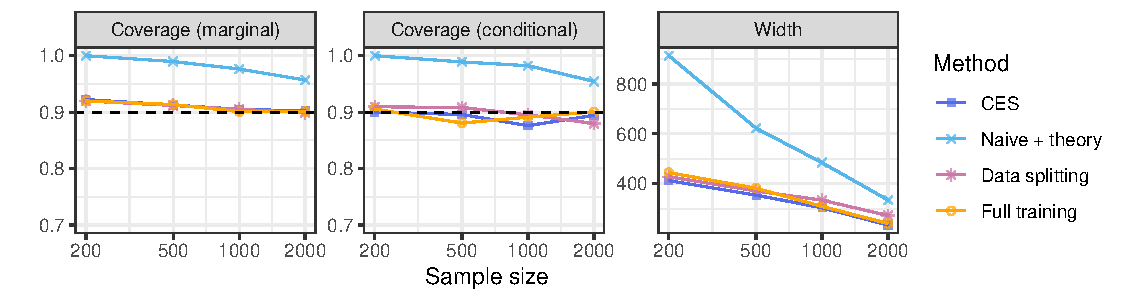
\includegraphics[width=0.8\linewidth]{figures/exp_regression_bike.pdf}
    \caption{Performance of conformal prediction intervals based on regression models trained with different methods, on the {\em bike} data set~\cite{data-bike}. The results are shown as a function of the total sample size. The nominal marginal coverage level is 90\%. See Table~\ref{fig:exp_regression_bike} for standard errors.}
    \label{fig:exp_regression_bike}
\end{figure}

\begin{figure}[!htb]
    \centering
    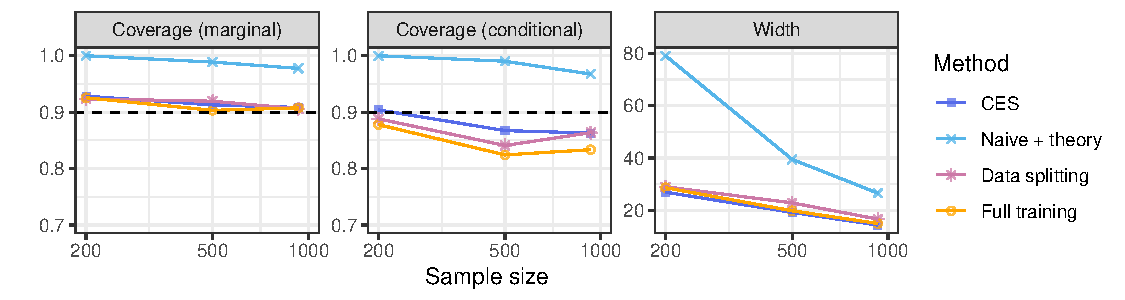
\includegraphics[width=0.8\linewidth]{figures/exp_regression_concrete.pdf}
    \caption{Performance of conformal prediction intervals based on regression models trained with different methods, on the {\em concrete} data set~\cite{data-concrete}. The results are shown as a function of the total sample size. The nominal marginal coverage level is 90\%. See Table~\ref{fig:exp_regression_concrete} for standard errors.}
    \label{fig:exp_regression_concrete}
\end{figure}


\begin{figure}[!htb]
    \centering
    \includegraphics[width=0.8\linewidth]{figures/exp_qt_regression_community.pdf}
    \caption{\color{blue} Performance of conformal prediction intervals based on quantile regression models trained with different methods, on the {\em community} data set~\cite{community}. The results are shown as a function of the total sample size with error bars corresponding to standard error. The nominal marginal coverage level is 90\%. See Table~\ref{tab:exp_qt_regression_community_tab} for more details.}
    \label{fig:exp_qt_regression_community}
\end{figure}

\begin{figure}[!htb]
    \centering
    \includegraphics[width=0.8\linewidth]{figures/exp_qt_regression_bio.pdf}
    \caption{\color{blue} Performance of conformal prediction intervals based on quantile regression models trained with different methods, on the {\em bio} data set~\cite{data-bio}. The results are shown as a function of the total sample size with error bars corresponding to standard error. The nominal marginal coverage level is 90\%. See Table~\ref{tab:exp_qt_regression_bio_tab} for more details.}
    \label{fig:exp_qt_regression_bio}
\end{figure}

\begin{figure}[!htb]
    \centering
    \includegraphics[width=0.8\linewidth]{figures/exp_qt_regression_meps_21.pdf}
    \caption{\color{blue} Performance of conformal prediction intervals based on quantile regression models trained with different methods, on the {\em meps\_21} data set~\cite{meps_21}.The results are shown as a function of the total sample size with error bars corresponding to standard error. The nominal marginal coverage level is 90\%. See Table~\ref{tab:exp_qt_regression_meps_21_tab} for more details.}
    \label{fig:exp_qt_regression_meps_21}
\end{figure}

\begin{figure}[!htb]
    \centering
    \includegraphics[width=0.8\linewidth]{figures/exp_qt_regression_blog_data.pdf}
    \caption{\color{blue} Performance of conformal prediction intervals based on quantile regression models trained with different methods, on the {\em blog\_data} data set~\cite{blog_data}. The results are shown as a function of the total sample size with error bars corresponding to standard error. The nominal marginal coverage level is 90\%. See Table~\ref{tab:exp_qt_regression_blog_data_tab} for more details.}
    \label{fig:exp_qt_regression_blog_data}
\end{figure}

\begin{figure}[!htb]
    \centering
    \includegraphics[width=0.8\linewidth]{figures/exp_qt_regression_star.pdf}
    \caption{\color{blue} Performance of conformal prediction intervals based on quantile regression models trained with different methods, on the {\em STAR} data set~\cite{star}. The results are shown as a function of the total sample size with error bars corresponding to standard error. The nominal marginal coverage level is 90\%. See Table~\ref{tab:exp_qt_regression_star_tab} for more details.}
    \label{fig:exp_qt_regression_star}
\end{figure}

\begin{figure}[!htb]
    \centering
    \includegraphics[width=0.8\linewidth]{figures/exp_qt_regression_bike.pdf}
    \caption{\color{blue} Performance of conformal prediction intervals based on quantile regression models trained with different methods, on the {\em bike} data set~\cite{data-bike}. The results are shown as a function of the total sample size with error bars corresponding to standard error. The nominal marginal coverage level is 90\%. See Table~\ref{tab:exp_qt_regression_bike_tab} for more details.}
    \label{fig:exp_qt_regression_bike}
\end{figure}



\begin{table}[!htb]
\centering
    \caption{Performance of outlier detection based on classification models trained with different methods, on the {\em CIFAR10} data set~\cite{cifar10}. Other details are as in Figure~\ref{fig:exp_oc}. The numbers in parenthesis indicate standard errors. The numbers in bold highlight TPR values within 1 standard error of the best TPR across all methods, for each sample size.}
  \label{tab:exp_oc}
  
\begin{tabular}{rlll}
\toprule
Sample size & Method & TPR & FPR\\
\midrule
\addlinespace[0.3em]
\multicolumn{4}{l}{\textbf{500}}\\
\hspace{1em}500 & CES & \textbf{0.296 (0.008)} & 0.098 (0.003)\\
\hspace{1em}500 & Naive + theory & 0.114 (0.006) & 0.016 (0.001)\\
\hspace{1em}500 & Data splitting & 0.234 (0.008) & 0.091 (0.003)\\
\hspace{1em}500 & Full training & 0.217 (0.011) & 0.072 (0.004)\\
\addlinespace[0.3em]
\multicolumn{4}{l}{\textbf{1000}}\\
\hspace{1em}1000 & CES & \textbf{0.401 (0.007)} & 0.100 (0.004)\\
\hspace{1em}1000 & Naive + theory & 0.237 (0.006) & 0.030 (0.002)\\
\hspace{1em}1000 & Data splitting & 0.337 (0.009) & 0.094 (0.003)\\
\hspace{1em}1000 & Full training & 0.189 (0.013) & 0.055 (0.004)\\
\addlinespace[0.3em]
\multicolumn{4}{l}{\textbf{2000}}\\
\hspace{1em}2000 & CES & \textbf{0.450 (0.005)} & 0.100 (0.003)\\
\hspace{1em}2000 & Naive + theory & 0.337 (0.006) & 0.048 (0.002)\\
\hspace{1em}2000 & Data splitting & 0.404 (0.007) & 0.095 (0.003)\\
\hspace{1em}2000 & Full training & 0.050 (0.009) & 0.017 (0.003)\\
\bottomrule
\end{tabular}

\end{table}

\begin{table}[!htb]
\centering
    \caption{Performance of multi-class classification based on classification models trained with different methods, on the {\em CIFAR10} data set~\cite{cifar10}. Other details are as in Figure~\ref{fig:exp_mc}. The numbers in parenthesis indicate standard errors. The numbers in bold highlight cardinality values within 1 standard error of the best cardinality across all methods, for each sample size.}
  \label{tab:exp_mc}
  
\begin{tabular}[t]{rlll}
\toprule
Sample size & Method & Cardinality & Marignal coverage\\
\midrule
\addlinespace[0.3em]
\multicolumn{4}{l}{\textbf{500}}\\
\hspace{1em}500 & CES & \textbf{6.754 (0.074)} & 0.908 (0.003)\\
\hspace{1em}500 & Naive & \textbf{6.735 (0.072)} & 0.906 (0.003)\\
\hspace{1em}500 & Naive + theory & 9.193 (0.052) & 0.988 (0.001)\\
\hspace{1em}500 & Data splitting & 7.022 (0.077) & 0.900 (0.004)\\
\hspace{1em}500 & Full training & \textbf{6.759 (0.091)} & 0.909 (0.004)\\
\addlinespace[0.3em]
\multicolumn{4}{l}{\textbf{1000}}\\
\hspace{1em}1000 & CES & \textbf{5.902 (0.060)} & 0.902 (0.003)\\
\hspace{1em}1000 & Naive & \textbf{5.908 (0.059)} & 0.901 (0.003)\\
\hspace{1em}1000 & Naive + theory & 7.767 (0.064) & 0.972 (0.002)\\
\hspace{1em}1000 & Data splitting & 6.294 (0.063) & 0.900 (0.004)\\
\hspace{1em}1000 & Full training & 6.270 (0.092) & 0.897 (0.004)\\
\addlinespace[0.3em]
\multicolumn{4}{l}{\textbf{2000}}\\
\hspace{1em}2000 & CES & \textbf{5.352 (0.045)} & 0.903 (0.003)\\
\hspace{1em}2000 & Naive & \textbf{5.347 (0.045)} & 0.902 (0.003)\\
\hspace{1em}2000 & Naive + theory & 6.609 (0.049) & 0.955 (0.002)\\
\hspace{1em}2000 & Data splitting & 5.674 (0.040) & 0.904 (0.003)\\
\hspace{1em}2000 & Full training & 7.776 (0.194) & 0.934 (0.006)\\
\bottomrule
\end{tabular}

\end{table}


\begin{table}[!htb]
\centering
    \caption{Performance of conformal prediction intervals based on regression models trained with different methods, on the {\em bio} data set~\cite{data-bio}. Other details are as in Figure~\ref{fig:exp_regression_bio}. The numbers in parenthesis indicate standard errors. The numbers in bold highlight width values within 1 standard error of the best width across all methods, for each sample size. The numbers in red highlight coverage values below 0.85.}
  \label{tab:exp_regression_bio}
  
\begin{tabular}{rlllll}
\toprule
\multicolumn{4}{c}{ } & \multicolumn{2}{c}{Coverage} \\
\cmidrule(l{3pt}r{3pt}){5-6}
Sample size & Data & Method & Width & Marginal & Conditional\\
\midrule
\addlinespace[0.3em]
\multicolumn{6}{l}{\textbf{200}}\\
\hspace{1em}200 & bio & CES & \textbf{18.740 (0.123)} & 0.924 (0.005) & 0.898 (0.014)\\
\hspace{1em}200 & bio & Naive + theory & 20.942 (0.006) & 1.000 (0.000) & 1.000 (0.000)\\
\hspace{1em}200 & bio & Data splitting & 19.068 (0.113) & 0.925 (0.005) & 0.902 (0.015)\\
\hspace{1em}200 & bio & Full training & \textbf{18.673 (0.125)} & 0.919 (0.004) & 0.890 (0.018)\\
\addlinespace[0.3em]
\multicolumn{6}{l}{\textbf{500}}\\
\hspace{1em}500 & bio & CES & \textbf{17.435 (0.125)} & 0.914 (0.004) & 0.909 (0.013)\\
\hspace{1em}500 & bio & Naive + theory & 20.391 (0.061) & 0.993 (0.001) & 0.996 (0.001)\\
\hspace{1em}500 & bio & Data splitting & 18.076 (0.123) & 0.911 (0.004) & 0.888 (0.015)\\
\hspace{1em}500 & bio & Full training & 18.245 (0.129) & 0.918 (0.003) & 0.890 (0.019)\\
\addlinespace[0.3em]
\multicolumn{6}{l}{\textbf{1000}}\\
\hspace{1em}1000 & bio & CES & \textbf{16.251 (0.081)} & 0.901 (0.003) & 0.885 (0.015)\\
\hspace{1em}1000 & bio & Naive + theory & 19.167 (0.073) & 0.977 (0.002) & 0.976 (0.006)\\
\hspace{1em}1000 & bio & Data splitting & 16.728 (0.089) & 0.903 (0.003) & 0.887 (0.016)\\
\hspace{1em}1000 & bio & Full training & 17.962 (0.141) & 0.902 (0.004) & \textcolor{red}{0.814 (0.022)}\\
\addlinespace[0.3em]
\multicolumn{6}{l}{\textbf{2000}}\\
\hspace{1em}2000 & bio & CES & \textbf{15.812 (0.042)} & 0.899 (0.003) & 0.893 (0.015)\\
\hspace{1em}2000 & bio & Naive + theory & 17.691 (0.047) & 0.957 (0.002) & 0.963 (0.006)\\
\hspace{1em}2000 & bio & Data splitting & 16.043 (0.059) & 0.900 (0.003) & 0.903 (0.015)\\
\hspace{1em}2000 & bio & Full training & 17.014 (0.113) & 0.902 (0.003) & \textcolor{red}{0.829 (0.019)}\\
\bottomrule
\end{tabular}

\end{table}

\begin{table}[!htb]
\centering
    \caption{Performance of conformal prediction intervals based on regression models trained with different methods, on the {\em bike} data set~\cite{data-bike}. Other details are as in Figure~\ref{fig:exp_regression_bike}. The numbers in parenthesis indicate standard errors. The numbers in bold highlight width values within 1 standard error of the best width across all methods, for each sample size. The numbers in red highlight coverage values below 0.85.}
  \label{tab:exp_regression_bike}
  \begin{tabular}[t]{rlllll}
\toprule
\multicolumn{4}{c}{ } & \multicolumn{2}{c}{Coverage} \\
\cmidrule(l{3pt}r{3pt}){5-6}
Sample size & Data & Method & Width & Marginal & Conditional\\
\midrule
\addlinespace[0.3em]
\multicolumn{6}{l}{\textbf{200}}\\
\hspace{1em}200 & bike & CES & 412.534 (6.439) & 0.922 (0.004) & 0.900 (0.018)\\
\hspace{1em}200 & bike & Naive & \textbf{392.474 (6.019)} & 0.908 (0.005) & 0.878 (0.016)\\
\hspace{1em}200 & bike & Naive + theory & 913.440 (3.737) & 1.000 (0.000) & 1.000 (0.000)\\
\hspace{1em}200 & bike & Data splitting & 427.964 (7.282) & 0.920 (0.004) & 0.910 (0.016)\\
\hspace{1em}200 & bike & Full training & 444.656 (6.760) & 0.920 (0.005) & 0.905 (0.013)\\
\addlinespace[0.3em]
\multicolumn{6}{l}{\textbf{500}}\\
\hspace{1em}500 & bike & CES & 354.180 (4.183) & 0.913 (0.004) & 0.896 (0.017)\\
\hspace{1em}500 & bike & Naive & \textbf{343.641 (4.220)} & 0.902 (0.004) & 0.889 (0.018)\\
\hspace{1em}500 & bike & Naive + theory & 622.837 (8.381) & 0.990 (0.001) & 0.989 (0.004)\\
\hspace{1em}500 & bike & Data splitting & 371.079 (3.777) & 0.912 (0.004) & 0.908 (0.014)\\
\hspace{1em}500 & bike & Full training & 381.951 (5.175) & 0.913 (0.004) & 0.881 (0.018)\\
\addlinespace[0.3em]
\multicolumn{6}{l}{\textbf{1000}}\\
\hspace{1em}1000 & bike & CES & \textbf{303.516 (3.047)} & 0.905 (0.004) & 0.876 (0.017)\\
\hspace{1em}1000 & bike & Naive & \textbf{300.091 (3.127)} & 0.903 (0.004) & 0.894 (0.015)\\
\hspace{1em}1000 & bike & Naive + theory & 484.565 (4.958) & 0.977 (0.002) & 0.982 (0.003)\\
\hspace{1em}1000 & bike & Data splitting & 333.939 (2.891) & 0.905 (0.003) & 0.895 (0.018)\\
\hspace{1em}1000 & bike & Full training & 308.981 (3.760) & 0.901 (0.004) & 0.891 (0.016)\\
\addlinespace[0.3em]
\multicolumn{6}{l}{\textbf{2000}}\\
\hspace{1em}2000 & bike & CES & \textbf{234.322 (1.935)} & 0.902 (0.003) & 0.894 (0.018)\\
\hspace{1em}2000 & bike & Naive & \textbf{231.571 (1.956)} & 0.897 (0.003) & 0.893 (0.018)\\
\hspace{1em}2000 & bike & Naive + theory & 334.724 (2.988) & 0.957 (0.002) & 0.954 (0.012)\\
\hspace{1em}2000 & bike & Data splitting & 272.589 (2.532) & 0.899 (0.003) & 0.880 (0.019)\\
\hspace{1em}2000 & bike & Full training & 240.714 (2.389) & 0.901 (0.003) & 0.901 (0.015)\\
\bottomrule
\end{tabular}

\end{table}

\begin{table}[!htb]
\centering
    \caption{Performance of conformal prediction intervals based on regression models trained with different methods, on the {\em concrete} data set~\cite{data-concrete}. Other details are as in Figure~\ref{fig:exp_regression_concrete}. The numbers in parenthesis indicate standard errors. The numbers in bold highlight width values within 1 standard error of the best width across all methods, for each sample size. The numbers in red highlight coverage values below 0.85.}
  \label{tab:exp_regression_concrete}
  \begin{tabular}[t]{rlllll}
\toprule
\multicolumn{4}{c}{ } & \multicolumn{2}{c}{Coverage} \\
\cmidrule(l{3pt}r{3pt}){5-6}
Sample size & Data & Method & Width & Marginal & Conditional\\
\midrule
\addlinespace[0.3em]
\multicolumn{6}{l}{\textbf{200}}\\
\hspace{1em}200 & concrete & CES & 26.948 (0.515) & 0.928 (0.005) & 0.904 (0.016)\\
\hspace{1em}200 & concrete & Naive & \textbf{24.793 (0.520)} & 0.903 (0.006) & 0.856 (0.021)\\
\hspace{1em}200 & concrete & Naive + theory & 79.089 (0.130) & 1.000 (0.000) & 1.000 (0.000)\\
\hspace{1em}200 & concrete & Data splitting & 29.021 (0.564) & 0.924 (0.004) & 0.888 (0.018)\\
\hspace{1em}200 & concrete & Full training & 28.676 (0.568) & 0.926 (0.005) & 0.878 (0.021)\\
\addlinespace[0.3em]
\multicolumn{6}{l}{\textbf{500}}\\
\hspace{1em}500 & concrete & CES & 19.232 (0.263) & 0.913 (0.004) & 0.867 (0.018)\\
\hspace{1em}500 & concrete & Naive & \textbf{18.340 (0.276)} & 0.896 (0.004) & \textcolor{red}{0.829 (0.022)}\\
\hspace{1em}500 & concrete & Naive + theory & 39.492 (0.861) & 0.989 (0.002) & 0.990 (0.003)\\
\hspace{1em}500 & concrete & Data splitting & 22.876 (0.323) & 0.919 (0.003) & \textcolor{red}{0.841 (0.023)}\\
\hspace{1em}500 & concrete & Full training & 19.857 (0.300) & 0.903 (0.004) & \textcolor{red}{0.824 (0.024)}\\
\addlinespace[0.3em]
\multicolumn{6}{l}{\textbf{930}}\\
\hspace{1em}930 & concrete & CES & 14.399 (0.134) & 0.908 (0.002) & 0.863 (0.014)\\
\hspace{1em}930 & concrete & Naive & \textbf{13.738 (0.127)} & 0.899 (0.002) & 0.863 (0.011)\\
\hspace{1em}930 & concrete & Naive + theory & 26.596 (0.334) & 0.978 (0.001) & 0.967 (0.004)\\
\hspace{1em}930 & concrete & Data splitting & 16.659 (0.122) & 0.906 (0.002) & 0.864 (0.014)\\
\hspace{1em}930 & concrete & Full training & 14.998 (0.143) & 0.908 (0.002) & \textcolor{red}{0.834 (0.016)}\\
\bottomrule
\end{tabular}

\end{table}


\begin{table}[!htb]
\centering
    \caption{\color{blue} Performance of conformal prediction intervals based on quantile regression models trained with different methods, on the {\em homes} data set~\cite{homes}. Other details are as in Figure~\ref{fig:exp_qt_regression_homes}. The numbers in parenthesis indicate standard errors. The numbers in bold highlight width values within 1 standard error of the best width across all methods, for each sample size. The numbers in red highlight coverage values below 0.85.}
    \label{tab:exp_qt_regression_homes_tab}
  
\begin{tabular}[t]{rlllll}
\toprule
\multicolumn{4}{c}{ } & \multicolumn{2}{c}{Coverage} \\
\cmidrule(l{3pt}r{3pt}){5-6}
Sample size & Data & Method & Width & Marginal & Conditional\\
\midrule
\addlinespace[0.3em]
\multicolumn{6}{l}{\textbf{200}}\\
\hspace{1em}200 & homes & CES & 1.396 (0.047) & 0.924 (0.007) & \textcolor{red}{0.804 (0.016)}\\
\hspace{1em}200 & homes & Naive + theory & 2.607 (0.222) & 0.983 (0.004) & 0.931 (0.015)\\
\hspace{1em}200 & homes & Data splitting & 1.329 (0.049) & 0.907 (0.006) & \textcolor{red}{0.730 (0.029)}\\
\hspace{1em}200 & homes & Full training & \textbf{1.195 (0.053)} & 0.919 (0.008) & \textcolor{red}{0.674 (0.030)}\\
\addlinespace[0.3em]
\multicolumn{6}{l}{\textbf{500}}\\
\hspace{1em}500 & homes & CES & 0.997 (0.022) & 0.909 (0.007) & \textcolor{red}{0.842 (0.016)}\\
\hspace{1em}500 & homes & Naive + theory & 2.698 (0.308) & 0.989 (0.003) & 0.950 (0.017)\\
\hspace{1em}500 & homes & Data splitting & 0.985 (0.019) & 0.896 (0.006) & \textcolor{red}{0.810 (0.020)}\\
\hspace{1em}500 & homes & Full training & \textbf{0.940 (0.043)} & 0.913 (0.007) & \textcolor{red}{0.710 (0.019)}\\
\addlinespace[0.3em]
\multicolumn{6}{l}{\textbf{1000}}\\
\hspace{1em}1000 & homes & CES & 0.858 (0.015) & 0.910 (0.005) & \textcolor{red}{0.827 (0.017)}\\
\hspace{1em}1000 & homes & Naive + theory & 1.229 (0.039) & 0.969 (0.004) & 0.917 (0.015)\\
\hspace{1em}1000 & homes & Data splitting & 0.926 (0.020) & 0.905 (0.004) & \textcolor{red}{0.786 (0.021)}\\
\hspace{1em}1000 & homes & Full training & \textbf{0.755 (0.019)} & 0.902 (0.005) & \textcolor{red}{0.698 (0.019)}\\
\addlinespace[0.3em]
\multicolumn{6}{l}{\textbf{2000}}\\
\hspace{1em}2000 & homes & CES & 0.726 (0.016) & 0.902 (0.005) & \textcolor{red}{0.824 (0.013)}\\
\hspace{1em}2000 & homes & Naive + theory & 0.865 (0.013) & 0.949 (0.003) & 0.880 (0.013)\\
\hspace{1em}2000 & homes & Data splitting & 0.779 (0.011) & 0.900 (0.003) & \textcolor{red}{0.804 (0.013)}\\
\hspace{1em}2000 & homes & Full training & \textbf{0.653 (0.013)} & 0.889 (0.005) & \textcolor{red}{0.686 (0.019)}\\
\bottomrule
\end{tabular}


\end{table}



\begin{table}[!htb]
\centering
    \caption{\color{blue} Performance of conformal prediction intervals based on quantile regression models trained with different methods, on the {\em community} data set~\cite{community}. Other details are as in Figure~\ref{fig:exp_qt_regression_community}. The numbers in parenthesis indicate standard errors. The numbers in bold highlight width values within 1 standard error of the best width across all methods, for each sample size. The numbers in red highlight coverage values below 0.85.}
    \label{tab:exp_qt_regression_community_tab}
  
\begin{tabular}[t]{rlllll}
\toprule
\multicolumn{4}{c}{ } & \multicolumn{2}{c}{Coverage} \\
\cmidrule(l{3pt}r{3pt}){5-6}
Sample size & Data & Method & Width & Marginal & Conditional\\
\midrule
\addlinespace[0.3em]
\multicolumn{6}{l}{\textbf{200}}\\
\hspace{1em}200 & community & CES & \textbf{2.226 (0.057)} & 0.905 (0.006) & \textcolor{red}{0.835 (0.018)}\\
\hspace{1em}200 & community & Naive + theory & 3.876 (0.193) & 0.980 (0.004) & 0.963 (0.008)\\
\hspace{1em}200 & community & Data splitting & \textbf{2.250 (0.081)} & 0.902 (0.007) & \textcolor{red}{0.811 (0.017)}\\
\hspace{1em}200 & community & Full training & 2.345 (0.070) & 0.903 (0.007) & \textcolor{red}{0.752 (0.023)}\\
\addlinespace[0.3em]
\multicolumn{6}{l}{\textbf{500}}\\
\hspace{1em}500 & community & CES & \textbf{1.957 (0.033)} & 0.902 (0.006) & \textcolor{red}{0.849 (0.014)}\\
\hspace{1em}500 & community & Naive + theory & 4.312 (0.254) & 0.990 (0.002) & 0.971 (0.008)\\
\hspace{1em}500 & community & Data splitting & 2.041 (0.037) & 0.904 (0.006) & \textcolor{red}{0.843 (0.011)}\\
\hspace{1em}500 & community & Full training & 2.084 (0.067) & 0.898 (0.007) & \textcolor{red}{0.770 (0.018)}\\
\addlinespace[0.3em]
\multicolumn{6}{l}{\textbf{994}}\\
\hspace{1em}994 & community & CES & \textbf{1.717 (0.016)} & 0.911 (0.003) & \textcolor{red}{0.850 (0.007)}\\
\hspace{1em}994 & community & Naive + theory & 2.486 (0.049) & 0.971 (0.002) & 0.943 (0.005)\\
\hspace{1em}994 & community & Data splitting & 1.818 (0.013) & 0.910 (0.002) & 0.865 (0.008)\\
\hspace{1em}994 & community & Full training & 1.784 (0.029) & 0.901 (0.003) & \textcolor{red}{0.797 (0.011)}\\
\bottomrule
\end{tabular}


\end{table}

\begin{table}[!htb]
\centering
    \caption{\color{blue} Performance of conformal prediction intervals based on quantile regression models trained with different methods, on the {\em bio} data set~\cite{data-bio}. Other details are as in Figure~\ref{fig:exp_qt_regression_bio}. The numbers in parenthesis indicate standard errors. The numbers in bold highlight width values within 1 standard error of the best width across all methods, for each sample size. The numbers in red highlight coverage values below 0.85.}
    \label{tab:exp_qt_regression_bio_tab}
  
\begin{tabular}[t]{rlllll}
\toprule
\multicolumn{4}{c}{ } & \multicolumn{2}{c}{Coverage} \\
\cmidrule(l{3pt}r{3pt}){5-6}
Sample size & Data & Method & Width & Marginal & Conditional\\
\midrule
\addlinespace[0.3em]
\multicolumn{6}{l}{\textbf{200}}\\
\hspace{1em}200 & bio & CES & 2.732 (0.074) & 0.926 (0.006) & \textcolor{red}{0.848 (0.022)}\\
\hspace{1em}200 & bio & Naive + theory & 3.392 (0.254) & 0.971 (0.005) & 0.954 (0.010)\\
\hspace{1em}200 & bio & Data splitting & \textbf{2.334 (0.083)} & 0.902 (0.010) & \textcolor{red}{0.803 (0.029)}\\
\hspace{1em}200 & bio & Full training & 2.848 (0.124) & 0.899 (0.010) & \textcolor{red}{0.844 (0.016)}\\
\addlinespace[0.3em]
\multicolumn{6}{l}{\textbf{500}}\\
\hspace{1em}500 & bio & CES & 2.154 (0.034) & 0.921 (0.004) & 0.872 (0.010)\\
\hspace{1em}500 & bio & Naive + theory & 3.893 (0.161) & 0.995 (0.001) & 0.996 (0.002)\\
\hspace{1em}500 & bio & Data splitting & \textbf{2.015 (0.024)} & 0.903 (0.004) & \textcolor{red}{0.840 (0.013)}\\
\hspace{1em}500 & bio & Full training & 2.579 (0.057) & 0.890 (0.011) & \textcolor{red}{0.819 (0.032)}\\
\addlinespace[0.3em]
\multicolumn{6}{l}{\textbf{1000}}\\
\hspace{1em}1000 & bio & CES & 1.997 (0.019) & 0.918 (0.004) & 0.890 (0.013)\\
\hspace{1em}1000 & bio & Naive + theory & 2.318 (0.033) & 0.969 (0.002) & 0.943 (0.010)\\
\hspace{1em}1000 & bio & Data splitting & \textbf{1.895 (0.018)} & 0.898 (0.006) & \textcolor{red}{0.811 (0.018)}\\
\hspace{1em}1000 & bio & Full training & 2.381 (0.035) & 0.877 (0.010) & \textcolor{red}{0.786 (0.037)}\\
\addlinespace[0.3em]
\multicolumn{6}{l}{\textbf{2000}}\\
\hspace{1em}2000 & bio & CES & 1.869 (0.018) & 0.906 (0.004) & 0.867 (0.016)\\
\hspace{1em}2000 & bio & Naive + theory & 1.998 (0.017) & 0.948 (0.003) & 0.922 (0.014)\\
\hspace{1em}2000 & bio & Data splitting & \textbf{1.830 (0.013)} & 0.898 (0.004) & 0.852 (0.015)\\
\hspace{1em}2000 & bio & Full training & 2.219 (0.029) & 0.874 (0.008) & \textcolor{red}{0.781 (0.035)}\\
\bottomrule
\end{tabular}


\end{table}


\begin{table}[!htb]
\centering
    \caption{\color{blue} Performance of conformal prediction intervals based on quantile regression models trained with different methods, on the {\em MEPS\_21} data set~\cite{meps_21}. Other details are as in Figure~\ref{fig:exp_qt_regression_meps_21}. The numbers in parenthesis indicate standard errors. The numbers in bold highlight width values within 1 standard error of the best width across all methods, for each sample size. The numbers in red highlight coverage values below 0.85.}
    \label{tab:exp_qt_regression_meps_21_tab}
  
\begin{tabular}[t]{rlllll}
\toprule
\multicolumn{4}{c}{ } & \multicolumn{2}{c}{Coverage} \\
\cmidrule(l{3pt}r{3pt}){5-6}
Sample size & Data & Method & Width & Marginal & Conditional\\
\midrule
\addlinespace[0.3em]
\multicolumn{6}{l}{\textbf{200}}\\
\hspace{1em}200 & meps\_21 & CES & 4.442 (0.468) & 0.927 (0.007) & \textcolor{red}{0.844 (0.020)}\\
\hspace{1em}200 & meps\_21 & Naive & \textbf{3.602 (0.452)} & 0.901 (0.010) & \textcolor{red}{0.786 (0.025)}\\
\hspace{1em}200 & meps\_21 & Naive + theory & 17.470 (2.874) & 0.979 (0.003) & 0.943 (0.012)\\
\hspace{1em}200 & meps\_21 & Data splitting & \textbf{3.239 (0.212)} & 0.909 (0.008) & \textcolor{red}{0.780 (0.021)}\\
\hspace{1em}200 & meps\_21 & Full training & 6.070 (0.509) & 0.906 (0.009) & \textcolor{red}{0.654 (0.030)}\\
\addlinespace[0.3em]
\multicolumn{6}{l}{\textbf{500}}\\
\hspace{1em}500 & meps\_21 & CES & 3.453 (0.074) & 0.912 (0.004) & \textcolor{red}{0.845 (0.015)}\\
\hspace{1em}500 & meps\_21 & Naive & \textbf{3.077 (0.068)} & 0.898 (0.005) & \textcolor{red}{0.802 (0.012)}\\
\hspace{1em}500 & meps\_21 & Naive + theory & 35.882 (4.705) & 0.991 (0.002) & 0.974 (0.008)\\
\hspace{1em}500 & meps\_21 & Data splitting & \textbf{3.147 (0.109)} & 0.906 (0.006) & \textcolor{red}{0.832 (0.012)}\\
\hspace{1em}500 & meps\_21 & Full training & 6.038 (0.305) & 0.913 (0.005) & \textcolor{red}{0.709 (0.021)}\\
\addlinespace[0.3em]
\multicolumn{6}{l}{\textbf{1000}}\\
\hspace{1em}1000 & meps\_21 & CES & 3.447 (0.068) & 0.896 (0.005) & \textcolor{red}{0.833 (0.012)}\\
\hspace{1em}1000 & meps\_21 & Naive & \textbf{3.102 (0.073)} & 0.888 (0.006) & \textcolor{red}{0.825 (0.014)}\\
\hspace{1em}1000 & meps\_21 & Naive + theory & 6.054 (0.443) & 0.970 (0.002) & 0.930 (0.009)\\
\hspace{1em}1000 & meps\_21 & Data splitting & \textbf{3.231 (0.093)} & 0.901 (0.005) & \textcolor{red}{0.817 (0.016)}\\
\hspace{1em}1000 & meps\_21 & Full training & 5.183 (0.188) & 0.902 (0.004) & \textcolor{red}{0.646 (0.019)}\\
\addlinespace[0.3em]
\multicolumn{6}{l}{\textbf{2000}}\\
\hspace{1em}2000 & meps\_21 & CES & 3.666 (0.054) & 0.907 (0.004) & 0.867 (0.012)\\
\hspace{1em}2000 & meps\_21 & Naive & \textbf{3.454 (0.047)} & 0.902 (0.004) & 0.875 (0.013)\\
\hspace{1em}2000 & meps\_21 & Naive + theory & 4.242 (0.069) & 0.951 (0.003) & 0.925 (0.010)\\
\hspace{1em}2000 & meps\_21 & Data splitting & \textbf{3.485 (0.060)} & 0.902 (0.003) & \textcolor{red}{0.847 (0.009)}\\
\hspace{1em}2000 & meps\_21 & Full training & 4.349 (0.128) & 0.897 (0.003) & \textcolor{red}{0.651 (0.018)}\\
\bottomrule
\end{tabular}

%%% Local Variables:
%%% mode: latex
%%% TeX-master: "../main"
%%% End:

\end{table}

\begin{table}[!htb]
\centering
    \caption{\color{blue} Performance of conformal prediction intervals based on quantile regression models trained with different methods, on the {\em blog\_data} data set~\cite{blog_data}. Other details are as in Figure~\ref{fig:exp_qt_regression_blog_data}. The numbers in parenthesis indicate standard errors. The numbers in bold highlight width values within 1 standard error of the best width across all methods, for each sample size. The numbers in red highlight coverage values below 0.85.}
    \label{tab:exp_qt_regression_blog_data_tab}
  
\begin{tabular}[t]{rlllll}
\toprule
\multicolumn{4}{c}{ } & \multicolumn{2}{c}{Coverage} \\
\cmidrule(l{3pt}r{3pt}){5-6}
Sample size & Data & Method & Width & Marginal & Conditional\\
\midrule
\addlinespace[0.3em]
\multicolumn{6}{l}{\textbf{200}}\\
\hspace{1em}200 & blog\_data & CES & 4.658 (0.194) & 0.911 (0.007) & \textcolor{red}{0.779 (0.021)}\\
\hspace{1em}200 & blog\_data & Naive + theory & 22.166 (5.645) & 0.973 (0.004) & 0.917 (0.017)\\
\hspace{1em}200 & blog\_data & Data splitting & \textbf{4.049 (0.359)} & 0.892 (0.013) & \textcolor{red}{0.720 (0.034)}\\
\hspace{1em}200 & blog\_data & Full training & 7.524 (0.544) & 0.910 (0.007) & \textcolor{red}{0.662 (0.026)}\\
\addlinespace[0.3em]
\multicolumn{6}{l}{\textbf{500}}\\
\hspace{1em}500 & blog\_data & CES & 4.538 (0.291) & 0.924 (0.005) & \textcolor{red}{0.819 (0.017)}\\
\hspace{1em}500 & blog\_data & Naive + theory & 58.965 (11.745) & 0.992 (0.002) & 0.987 (0.004)\\
\hspace{1em}500 & blog\_data & Data splitting & \textbf{3.443 (0.139)} & 0.905 (0.005) & \textcolor{red}{0.751 (0.020)}\\
\hspace{1em}500 & blog\_data & Full training & 9.364 (0.535) & 0.927 (0.003) & \textcolor{red}{0.719 (0.019)}\\
\addlinespace[0.3em]
\multicolumn{6}{l}{\textbf{1000}}\\
\hspace{1em}1000 & blog\_data & CES & 4.313 (0.088) & 0.903 (0.004) & \textcolor{red}{0.812 (0.016)}\\
\hspace{1em}1000 & blog\_data & Naive + theory & 7.336 (0.620) & 0.973 (0.002) & 0.951 (0.007)\\
\hspace{1em}1000 & blog\_data & Data splitting & \textbf{3.525 (0.119)} & 0.896 (0.003) & \textcolor{red}{0.788 (0.015)}\\
\hspace{1em}1000 & blog\_data & Full training & 7.784 (0.427) & 0.919 (0.003) & \textcolor{red}{0.694 (0.018)}\\
\addlinespace[0.3em]
\multicolumn{6}{l}{\textbf{2000}}\\
\hspace{1em}2000 & blog\_data & CES & 4.169 (0.066) & 0.906 (0.003) & \textcolor{red}{0.808 (0.013)}\\
\hspace{1em}2000 & blog\_data & Naive + theory & 4.486 (0.074) & 0.954 (0.002) & 0.911 (0.009)\\
\hspace{1em}2000 & blog\_data & Data splitting & \textbf{3.625 (0.069)} & 0.899 (0.003) & \textcolor{red}{0.805 (0.011)}\\
\hspace{1em}2000 & blog\_data & Full training & 5.323 (0.274) & 0.909 (0.003) & \textcolor{red}{0.718 (0.014)}\\
\bottomrule
\end{tabular}


\end{table}


\begin{table}[!htb]
\centering
    \caption{\color{blue} Performance of conformal prediction intervals based on quantile regression models trained with different methods, on the {\em STAR} data set~\cite{star}. Other details are as in Figure~\ref{fig:exp_qt_regression_star}. The numbers in parenthesis indicate standard errors. The numbers in bold highlight width values within 1 standard error of the best width across all methods, for each sample size. The numbers in red highlight coverage values below 0.85.}
    \label{tab:exp_qt_regression_star_tab}
  
\begin{tabular}[t]{rlllll}
\toprule
\multicolumn{4}{c}{ } & \multicolumn{2}{c}{Coverage} \\
\cmidrule(l{3pt}r{3pt}){5-6}
Sample size & Data & Method & Width & Marginal & Conditional\\
\midrule
\addlinespace[0.3em]
\multicolumn{6}{l}{\textbf{200}}\\
\hspace{1em}200 & star & CES & 0.567 (0.023) & 0.933 (0.006) & 0.891 (0.012)\\
\hspace{1em}200 & star & Naive & 0.421 (0.031) & 0.904 (0.008) & \textcolor{red}{0.847 (0.012)}\\
\hspace{1em}200 & star & Naive + theory & 0.656 (0.038) & 0.984 (0.002) & 0.960 (0.006)\\
\hspace{1em}200 & star & Data splitting & 0.502 (0.022) & 0.911 (0.009) & 0.862 (0.013)\\
\hspace{1em}200 & star & Full training & \textbf{0.323 (0.008)} & 0.914 (0.006) & 0.872 (0.012)\\
\addlinespace[0.3em]
\multicolumn{6}{l}{\textbf{500}}\\
\hspace{1em}500 & star & CES & 0.318 (0.007) & 0.929 (0.004) & 0.893 (0.012)\\
\hspace{1em}500 & star & Naive & 0.288 (0.008) & 0.902 (0.007) & \textcolor{red}{0.848 (0.016)}\\
\hspace{1em}500 & star & Naive + theory & 0.520 (0.025) & 0.992 (0.001) & 0.978 (0.005)\\
\hspace{1em}500 & star & Data splitting & 0.328 (0.009) & 0.910 (0.006) & 0.860 (0.015)\\
\hspace{1em}500 & star & Full training & \textbf{0.224 (0.005)} & 0.909 (0.006) & 0.874 (0.013)\\
\addlinespace[0.3em]
\multicolumn{6}{l}{\textbf{1000}}\\
\hspace{1em}1000 & star & CES & 0.252 (0.005) & 0.914 (0.003) & 0.864 (0.012)\\
\hspace{1em}1000 & star & Naive & 0.236 (0.007) & 0.897 (0.003) & 0.862 (0.011)\\
\hspace{1em}1000 & star & Naive + theory & 0.323 (0.007) & 0.967 (0.003) & 0.929 (0.009)\\
\hspace{1em}1000 & star & Data splitting & 0.269 (0.007) & 0.903 (0.003) & \textcolor{red}{0.846 (0.012)}\\
\hspace{1em}1000 & star & Full training & \textbf{0.182 (0.002)} & 0.898 (0.004) & \textcolor{red}{0.848 (0.012)}\\
\addlinespace[0.3em]
\multicolumn{6}{l}{\textbf{1161}}\\
\hspace{1em}1161 & star & CES & 0.237 (0.005) & 0.920 (0.004) & 0.882 (0.012)\\
\hspace{1em}1161 & star & Naive & 0.220 (0.005) & 0.900 (0.005) & 0.860 (0.012)\\
\hspace{1em}1161 & star & Naive + theory & 0.308 (0.007) & 0.969 (0.002) & 0.944 (0.007)\\
\hspace{1em}1161 & star & Data splitting & 0.254 (0.007) & 0.903 (0.004) & 0.864 (0.014)\\
\hspace{1em}1161 & star & Full training & \textbf{0.174 (0.003)} & 0.896 (0.004) & 0.863 (0.013)\\
\bottomrule
\end{tabular}


\end{table}

\begin{table}[!htb]
\centering
    \caption{\color{blue} Performance of conformal prediction intervals based on quantile regression models trained with different methods, on the {\em bike} data set~\cite{data-bike}. Other details are as in Figure~\ref{fig:exp_qt_regression_bike}. The numbers in parenthesis indicate standard errors. The numbers in bold highlight width values within 1 standard error of the best width across all methods, for each sample size. The numbers in red highlight coverage values below 0.85.}
    \label{tab:exp_qt_regression_bike_tab}
  \begin{tabular}[t]{rlllll}
\toprule
\multicolumn{4}{c}{ } & \multicolumn{2}{c}{Coverage} \\
\cmidrule(l{3pt}r{3pt}){5-6}
Sample size & Data & Method & Width & Marginal & Conditional\\
\midrule
\addlinespace[0.3em]
\multicolumn{6}{l}{\textbf{200}}\\
\hspace{1em}200 & bike & CES & \textbf{2.690 (0.065)} & 0.923 (0.006) & 0.895 (0.014)\\
\hspace{1em}200 & bike & Naive + theory & 4.106 (0.192) & 0.979 (0.003) & 0.958 (0.008)\\
\hspace{1em}200 & bike & Data splitting & \textbf{2.663 (0.056)} & 0.899 (0.008) & \textcolor{red}{0.832 (0.018)}\\
\hspace{1em}200 & bike & Full training & 2.843 (0.095) & 0.910 (0.006) & 0.870 (0.012)\\
\addlinespace[0.3em]
\multicolumn{6}{l}{\textbf{500}}\\
\hspace{1em}500 & bike & CES & \textbf{2.244 (0.039)} & 0.913 (0.004) & 0.886 (0.014)\\
\hspace{1em}500 & bike & Naive + theory & 4.284 (0.152) & 0.991 (0.002) & 0.984 (0.005)\\
\hspace{1em}500 & bike & Data splitting & \textbf{2.275 (0.032)} & 0.902 (0.004) & 0.859 (0.014)\\
\hspace{1em}500 & bike & Full training & \textbf{2.265 (0.062)} & 0.908 (0.004) & \textcolor{red}{0.839 (0.014)}\\
\addlinespace[0.3em]
\multicolumn{6}{l}{\textbf{1000}}\\
\hspace{1em}1000 & bike & CES & 1.978 (0.036) & 0.911 (0.004) & 0.872 (0.013)\\
\hspace{1em}1000 & bike & Naive + theory & 2.590 (0.061) & 0.968 (0.002) & 0.955 (0.007)\\
\hspace{1em}1000 & bike & Data splitting & 1.996 (0.040) & 0.903 (0.004) & 0.852 (0.013)\\
\hspace{1em}1000 & bike & Full training & \textbf{1.625 (0.045)} & 0.901 (0.005) & 0.858 (0.013)\\
\addlinespace[0.3em]
\multicolumn{6}{l}{\textbf{2000}}\\
\hspace{1em}2000 & bike & CES & 1.262 (0.030) & 0.902 (0.003) & 0.854 (0.012)\\
\hspace{1em}2000 & bike & Naive + theory & 1.570 (0.033) & 0.948 (0.003) & 0.933 (0.009)\\
\hspace{1em}2000 & bike & Data splitting & 1.517 (0.033) & 0.893 (0.003) & 0.853 (0.011)\\
\hspace{1em}2000 & bike & Full training & \textbf{1.061 (0.019)} & 0.887 (0.004) & \textcolor{red}{0.839 (0.013)}\\
\bottomrule
\end{tabular}


\end{table}


\clearpage

\section{Mathematical proofs} \label{appendix:proofs}

\begin{proof}[Proof of Theorem \ref{thm:od_full}]
It suffices to show that the nonconformity scores $\hat{S}_i$ for $i \in \{n+1\}\cup \mathcal{D}_{\text{es-cal}}$ are exchangeable. In fact, if the nonconformity scores are almost-surely unique, this implies the rank of $\hat{S}_{n+1}$ is uniformly distributed over $\{\hat{S}_{i}\}_{i \in \{n+1\}\cup \mathcal{D}_{\text{es-cal}}}$, and in that case the conformal p-value is uniformly distributed over $\{ 1/(1+|\mathcal{D}_{\text{es-cal}}|), 2/(1+|\mathcal{D}_{\text{es-cal}}|), \dots, 1\}$. If the nonconformity scores are not almost-surely unique and ties are not broken at random, then the distribution of the conformal p-value becomes stochastically larger than uniform, in which case the result still holds.
To prove the exchangeability of the nonconformity scores, let $\sigma$ be any permutation of $\{n+1\}\cup \mathcal{D}_{\text{es-cal}}$, and imagine applying Algorithm~\ref{alg:od_full_seq}, with the same random seed, to the shuffled data set indexed by $\sigma(\{n+1\}\cup \mathcal{D}_{\text{es-cal}})$, which has the same distribution as the original data set. To clarify the notation, we will refer to quantities computed under this data shuffling scenario with their usual symbol followed by an apostrophe; i.e., $M'_{t_1}$ instead of $M_{t_1}$.
As the gradient updates only involve the unperturbed observations in $\mathcal{D}_{\text{train}}$ and the maximum number of epochs $t^{\text{max}}$ is fixed, the sequence of saved models remains exactly the same under this scenario: $(M'_{t_1} , \dots, M'_{t_T}) = (M_{t_1} , \dots, M_{t_T})$.
Further, the loss function in~\eqref{eq:loss-ces} is also invariant to permutations of $\{n+1\}\cup \mathcal{D}_{\text{es-cal}}$, in the sense that $\mathcal{L}_{\text{es-cal}}^{+1'} = \mathcal{L}_{\text{es-cal}}^{+1}$, because $\mathcal{L}$ is additive.
Therefore, the model selected according to \eqref{eq:ces-model} is also invariant, $\hat{M}'_{\text{ces}} = \hat{M}_{\text{ces}}$, which implies the nonconformity scores are simply re-ordered: $\hat{S}'_{\sigma(i)} = \hat{S}_{i}$.
Therefore, we have:
\begin{align*}
  \sigma(\{\hat{S}_i\}_{i \in \{n+1\}\cup \mathcal{D}_{\text{cal}}})
  &= \{\hat{S}'_i\}_{i \in \{n+1\}\cup \mathcal{D}_{\text{cal}}} \\
  & \overset{d}{=} \{\hat{S}_i\}_{i \in \{n+1\}\cup \mathcal{D}_{\text{cal}}},
\end{align*}
where the last equality follows from the initial data exchangeability assumption.
\end{proof}

\begin{proof}[Proof of Theorem \ref{thm:class_full}]
Note that, conditional on $Y_{n+1}=y$, the miscoverage event $Y_{n+1} \not\in \hat{\mathcal{C}}_{\alpha}(X_{n+1})$ occurs if and only if $\hat{u}_y(X_{n+1}) \leq \alpha$, where $\hat{u}_y(X_{n+1})$ is defined as in~\eqref{eq:conformal_pval-class}.
Therefore, it suffices to show $\mathbb{P}\left[\hat{u}_y(X_{n+1}) \leq \alpha \mid Y_{n+1}=y\right] \leq \alpha$ for any $\alpha \in (0,1)$.
However, this is directly implied by Theorem \ref{thm:od_full}, because the $\hat{u}_y(X_{n+1})$ calculated by Algorithm~\ref{alg:class_full_seq} is equivalent to the conformal p-value $\hat{u}_0(Z_{n+1})$ given by Algorithm~\ref{alg:od_full_seq} applied to the subset of the data in $\mathcal{D}_{\text{es-cal}}$ with $Y_{i} = y$, with the understanding that $Z_i=(X_i,Y_i)$ for all $i \in \{n+1\} \cup \mathcal{D}_{\text{es-cal}}$.
\end{proof}

\begin{proof}[Proof of Theorem \ref{thm:class_full_marg}]
Note that $Y_{n+1} \not\in \hat{\mathcal{C}}^{\text{m}}_{\alpha}(X_{n+1})$ if and only if $\hat{u}^{\text{marg}}(X_{n+1};Y_{n+1}) \leq \alpha$, where $\hat{u}^{\text{marg}}(X_{n+1};Y_{n+1})$ is defined as in~\eqref{eq:conformal_pval-class_marg}. Hence it suffices to show that $\mathbb{P}\left[\hat{u}^{\text{marg}}(X_{n+1};Y_{n+1}) \leq \alpha \right] \leq \alpha$ for any $\alpha \in (0,1)$.
This can be established using the same approach as in the proof of Theorem~\ref{thm:od_full}, setting $Z_i=(X_i,Y_i)$ for all $i \in \{n+1\} \cup \mathcal{D}_{\text{es-cal}}$.
In fact, the maximum number of epochs $t^{\text{max}}$ is fixed, the sequence of saved models is invariant to permutations of $\{n+1\} \cup \mathcal{D}_{\text{es-cal}}$, and the model $\hat{M}_{\text{ces}}$ selected according to \eqref{eq:ces-model-class} is also invariant.
Thus, it follows that the nonconformity scores $\hat{S}_i$ are exchangeable with one another for all $i \in \{n+1\} \cup \mathcal{D}_{\text{es-cal}}$.
\end{proof}

\begin{proof}[Proof of Theorem \ref{thm:reg}]
Consider an imaginary oracle algorithm producing an interval $\hat{C}^{\text{oracle}}_{\alpha}(X_{n+1})$ defined as $\hat{C}^{\text{oracle}}_{\alpha}(X_{n+1}) = \mathcal{B}_{l^*(Y_{n+1})} \bigcap \hat{C}_{\alpha}(X_{n+1}, \mathcal{B}_{l^*(Y_{n+1})})$, where $l^*(Y_{n+1})$ is the exact index of the bin $\mathcal{B}_l$ to which the true $Y_{n+1}$ belongs. Clearly, this oracle is just a theoretical tool, not a practical method because the outcome value for the test point is unknown.
However, this oracle is useful because it is easier to analyze, and it suffices to establish that $\mathbb{P}[Y_{n+1} \in \hat{C}^{\text{oracle}}_{\alpha}(X_{n+1})] \geq 1-\alpha$, for any $\alpha \in (0,1)$, since $\hat{C}_{\alpha}(X_{n+1}) \supseteq \hat{C}^{\text{oracle}}_{\alpha}(X_{n+1})$ almost-surely.
The coverage property for the oracle can be established using an approach similar to that of the proof of Theorem~\ref{thm:od_full}, setting $Z_i=(X_i,Y_i)$ for all $i \in \{n+1\} \cup \mathcal{D}_{\text{es-cal}}$.
In fact, the maximum number of epochs $t^{\text{max}}$ is fixed, the sequence of saved models is invariant to permutations of $\{n+1\} \cup \mathcal{D}_{\text{es-cal}}$, and the  model $\hat{M}_{\text{ces}}$ selected by the oracle according to \eqref{eq:reg-step-func} is also invariant.
Thus, it follows that the oracle nonconformity scores $\hat{S}_i^* = \hat{S}_i(X_{n+1}, \mathcal{B}_{l^*(Y_{n+1})})$ are exchangeable with one another for all $i \in \{n+1\} \cup \mathcal{D}_{\text{es-cal}}$.
Further, by construction of the prediction intervals~\eqref{eq:reg-int-tmp}, we know that the miscoverage event $Y_{n+1} \not\in \hat{C}^{\text{oracle}}_{\alpha}(X_{n+1})$ occurs if and only if $\hat{S}^*_i > \hat{Q}^*_{1-\alpha}$, where $\hat{Q}^*_{1-\alpha}$ is the $\lceil (1-\alpha)(1+|\mathcal{D}_{\text{es-cal}}|) \rceil$-th largest value among all nonconformity scores $\hat{S}_i(X_{n+1},\mathcal{B}_l)$.
However, it is a well-known exchangeability result that $\mathbb{P}[\hat{S}^*_i \leq \hat{Q}^*_{1-\alpha}] \geq 1-\alpha$; see for example Lemma 1 in \citet{romano2019conformalized}.
\end{proof}


\begin{proof}[Proof of Theorem \ref{thm:reg-cqr}]
Same as the proof above. 
\end{proof}

\begin{proof}[Proof of Corollary~\ref{thm:reg-noempty}]
This corollary follows immediately from Theorem~\ref{thm:reg} because the prediction interval given by Algorithm~\ref{alg:reg-noempty} is always contained in that output by Algorithm~\ref{alg:reg}.
\end{proof}


\begin{proof}[Proof of Proposition~\ref{prop:naive-od}]
Note that $\hat{u}_0^{\textup{naive}}(Z_{n+1}) = \hat{u}_0^{\textup{naive}}(Z_{n+1};t^*)$, hence
    \begin{align*}
        \P{\hat{u}_0^{\textup{naive}}(Z_{n+1}) > \alpha} &= \mathbb{E} \bigl [\P{\hat{u}_0^{\textup{naive}}(Z_{n+1};t^*) > \alpha \mid \mathcal{D}_{\text{es-cal}}} \bigr ] \\
        &\geq \E{\min_{t\in [T]} W_t}        \\
        & \geq \sup_{a \in [0,1]} a \cdot \P{\min_{t\in [T]} W_t \geq a}\\
        &= \sup_{a \in [0,1]} a \left(1-\P{\min_{t\in [T]} W_t \leq a} \right)  \\
        &\geq \sup_{a \in [0,1]} a \left(1-T \cdot \P{W_t \leq a} \right),
   \end{align*}
where the last inequality follows from a union bound. To simplify the right-hand-side term above, let $a= I^{-1} \left(\frac{1}{bT};n_{\text{es-cal}}+1-l,l \right)$, where $b$ is any large constant. Hence we obtain
\begin{align*}
    \P{\hat{u}_0^{\textup{naive}}(Z_{n+1}) > \alpha} \geq I^{-1} \left(\frac{1}{bT};n_{\text{es-cal}}+1-l,l \right) \cdot (1-1/b).
\end{align*}
\end{proof}

\begin{proof}[Proof of Corollary~\ref{prop:naive-class}]
   Note that $Y_{n+1} \in \hat{C}^{\textup{naive}}_{\alpha}(X_{n+1})$ if and only if $\hat{u}^{\textup{naive}}_{Y_{n+1}}(X_{n+1};t^*) > \alpha$. Let $W_t$ denote the calibration conditional coverage $\P{\hat{u}^{\textup{naive}}_{Y_{n+1}}(X_{n+1};t) > \alpha \mid \mathcal{D}_{\text{es-cal}}}$. Then, we have
   \begin{align*}
       \P{Y_{n+1} \in \hat{C}^{\textup{naive}}_{\alpha}(X_{n+1})}
     = \mathbb{E}\left [\P{\hat{u}^{\textup{naive}}_{Y_{n+1}}(X_{n+1};t^*) > \alpha \mid \mathcal{D}_{\text{es-cal}}} \right ]
       = \E{W_{t^*}} \geq \E{\min_{t\in [T]} W_t}.
   \end{align*}
The rest of the proof follows the same argument as in the proof of Proposition \ref{prop:naive-od}.
\end{proof}

\begin{proof}[Proof of Corollary~\ref{prop:naive-reg}]
    Let $\hat{S}_i(X_{n+1}, t) = | Y_i - \hat{\mu}_{t}(X_i)|$ denote the residual score calculated with model $t \in [T]$, for all $i \in \mathcal{D}_{\text{es-cal}} $. Note that $Y_{n+1} \in \hat{C}^{\textup{naive}}_{\alpha}(X_{n+1})$ if and only if $\hat{S}_{X_{n+1}}(X_{n+1}, t^*) \leq \hat{Q}_{1-\alpha}$. Then, we just need to bound $W_t=\P{ \hat{S}_{X_{n+1}}(X_{n+1}, t^*) \leq \hat{Q}_{1-\alpha} \mid \mathcal{D}_{\text{es-cal}}}$, and the rest of the proof follows the same steps as the proof of Proposition~\ref{prop:naive-od}.
\end{proof}



%%% Local Variables:
%%% mode: latex
%%% TeX-master: "main"
%%% End:
